\documentclass[twoside]{book}

% Packages required by doxygen
\usepackage{fixltx2e}
\usepackage{calc}
\usepackage{doxygen}
\usepackage[export]{adjustbox} % also loads graphicx
\usepackage{graphicx}
\usepackage[utf8]{inputenc}
\usepackage{makeidx}
\usepackage{multicol}
\usepackage{multirow}
\PassOptionsToPackage{warn}{textcomp}
\usepackage{textcomp}
\usepackage[nointegrals]{wasysym}
\usepackage[table]{xcolor}

% Font selection
\usepackage[T1]{fontenc}
\usepackage[scaled=.90]{helvet}
\usepackage{courier}
\usepackage{amssymb}
\usepackage{sectsty}
\renewcommand{\familydefault}{\sfdefault}
\allsectionsfont{%
  \fontseries{bc}\selectfont%
  \color{darkgray}%
}
\renewcommand{\DoxyLabelFont}{%
  \fontseries{bc}\selectfont%
  \color{darkgray}%
}
\newcommand{\+}{\discretionary{\mbox{\scriptsize$\hookleftarrow$}}{}{}}

% Page & text layout
\usepackage{geometry}
\geometry{%
  a4paper,%
  top=2.5cm,%
  bottom=2.5cm,%
  left=2.5cm,%
  right=2.5cm%
}
\tolerance=750
\hfuzz=15pt
\hbadness=750
\setlength{\emergencystretch}{15pt}
\setlength{\parindent}{0cm}
\setlength{\parskip}{3ex plus 2ex minus 2ex}
\makeatletter
\renewcommand{\paragraph}{%
  \@startsection{paragraph}{4}{0ex}{-1.0ex}{1.0ex}{%
    \normalfont\normalsize\bfseries\SS@parafont%
  }%
}
\renewcommand{\subparagraph}{%
  \@startsection{subparagraph}{5}{0ex}{-1.0ex}{1.0ex}{%
    \normalfont\normalsize\bfseries\SS@subparafont%
  }%
}
\makeatother

% Headers & footers
\usepackage{fancyhdr}
\pagestyle{fancyplain}
\fancyhead[LE]{\fancyplain{}{\bfseries\thepage}}
\fancyhead[CE]{\fancyplain{}{}}
\fancyhead[RE]{\fancyplain{}{\bfseries\leftmark}}
\fancyhead[LO]{\fancyplain{}{\bfseries\rightmark}}
\fancyhead[CO]{\fancyplain{}{}}
\fancyhead[RO]{\fancyplain{}{\bfseries\thepage}}
\fancyfoot[LE]{\fancyplain{}{}}
\fancyfoot[CE]{\fancyplain{}{}}
\fancyfoot[RE]{\fancyplain{}{\bfseries\scriptsize Generated by Doxygen }}
\fancyfoot[LO]{\fancyplain{}{\bfseries\scriptsize Generated by Doxygen }}
\fancyfoot[CO]{\fancyplain{}{}}
\fancyfoot[RO]{\fancyplain{}{}}
\renewcommand{\footrulewidth}{0.4pt}
\renewcommand{\chaptermark}[1]{%
  \markboth{#1}{}%
}
\renewcommand{\sectionmark}[1]{%
  \markright{\thesection\ #1}%
}

% Indices & bibliography
\usepackage{natbib}
\usepackage[titles]{tocloft}
\setcounter{tocdepth}{3}
\setcounter{secnumdepth}{5}
\makeindex

% Hyperlinks (required, but should be loaded last)
\usepackage{ifpdf}
\ifpdf
  \usepackage[pdftex,pagebackref=true]{hyperref}
\else
  \usepackage[ps2pdf,pagebackref=true]{hyperref}
\fi
\hypersetup{%
  colorlinks=true,%
  linkcolor=blue,%
  citecolor=blue,%
  unicode%
}

% Custom commands
\newcommand{\clearemptydoublepage}{%
  \newpage{\pagestyle{empty}\cleardoublepage}%
}

\usepackage{caption}
\captionsetup{labelsep=space,justification=centering,font={bf},singlelinecheck=off,skip=4pt,position=top}

%===== C O N T E N T S =====

\begin{document}

% Titlepage & ToC
\hypersetup{pageanchor=false,
             bookmarksnumbered=true,
             pdfencoding=unicode
            }
\pagenumbering{roman}
\begin{titlepage}
\vspace*{7cm}
\begin{center}%
{\Large Human Detection Module }\\
\vspace*{1cm}
{\large Generated by Doxygen 1.8.11}\\
\end{center}
\end{titlepage}
\clearemptydoublepage
\tableofcontents
\clearemptydoublepage
\pagenumbering{arabic}
\hypersetup{pageanchor=true}

%--- Begin generated contents ---
\chapter{Human Detection Module}
\label{md_readme}
\hypertarget{md_readme}{}
\href{https://travis-ci.org/urastogi885/humanDetectionModule}{\tt } \subsection*{\href{https://coveralls.io/github/urastogi885/humanDetectionModule?branch=master}{\tt } }

\subsection*{Overview}

Human Detection module for A\+C\+ME Robotics with\+:


\begin{DoxyItemize}
\item cmake
\item googletest
\end{DoxyItemize}

We are designing a new human detection module by incorporating high-\/quality software engineering practices for Acme Robotics to take our deliverable, finish development, and integrate it into their product.

Detection and avoidance of human obstacles play a crucial role in any self-\/driving system. The design and development of real-\/time obstacle detection systems are currently one of the most demanding components in the autonomous industry. To address real-\/life problems involved in obstacle detection, a plethora of sensors such as L\+I\+D\+A\+Rs, Radars, and cameras, are being used in the industry. We are making use of the most readily available resource, images, to identify human obstacles.

Our module will be able to identify multiple humans in an image. The final deliverable of our module will be a set of images with location information of the detected humans. The robot\textquotesingle{}s system will be able to use this location information. We are assuming the input and output of our module to be a set of static images.

The module is still under development. After the final stage of development, the module will be capable of detecting multiple humans within a frame. We will add results and performance examples by the end of phase 2.

\subsection*{Team Members}

All of the team members are pursuing M.\+Eng. in Robotics at the University of Maryland.


\begin{DoxyItemize}
\item Umang Rastogi -\/ B.\+Tech in Electronics \& Communication Engineering
\item Aruna Baijal -\/ B.\+Tech in Computer Science \& Engineering
\item Achal Vyas -\/ B.\+Tech in Mechanical Engineering
\end{DoxyItemize}

\subsection*{License}


\begin{DoxyItemize}
\item This module has been developed under the 3-\/\+Clause B\+SD License.
\item Please go through the \href{https://github.com/urastogi885/humanDetectionModule/blob/phase1/LICENSE}{\tt {\itshape L\+I\+C\+E\+N\+SE}} file before cloning the repository.
\end{DoxyItemize}

\subsection*{A\+IP and Sprint Documents}


\begin{DoxyItemize}
\item Click on this \href{https://docs.google.com/spreadsheets/d/1oHHijKNsoFVp84mNC5g5sJ4BwJQwT6XpO5uRFw9AMzE/edit?usp=sharing}{\tt {\itshape link}} to access our A\+IP Google Sheet.
\item Click on this \href{https://docs.google.com/document/d/13PsjxV7XgBc0alKm0SCArrKI3s-3ExToed2AtDfnuaQ/edit?usp=sharing}{\tt {\itshape link}} to access our Sprint notes document.
\end{DoxyItemize}

\subsection*{Install Open\+CV}


\begin{DoxyItemize}
\item The module utilizes features of Open\+CV.
\item Although the repository contains Open\+CV library under the vendor directory, please update you system with necessary dependencies.
\item Run the commands below to install Open\+CV dependencies before cloning the repository\+: 
\begin{DoxyCode}
1 sudo apt-get install build-essential
2 sudo apt-get install cmake git libgtk2.0-dev pkg-config libavcodec-dev libavformat-dev libswscale-dev
3 sudo apt-get install python-dev python-numpy libtbb2 libtbb-dev libjpeg-dev libpng-dev libtiff-dev
       libjasper-dev libdc1394-22-dev
\end{DoxyCode}

\end{DoxyItemize}

\subsection*{Standard install via command-\/line}


\begin{DoxyItemize}
\item Switch to the directory where you want to clone this repository
\item Run the following command\+: 
\begin{DoxyCode}
1 git clone --recursive https://travis-ci.org/urastogi885/humanDetectionModule
2 mkdir build
3 cd build/
4 cmake ..
5 make
\end{DoxyCode}

\end{DoxyItemize}

\subsection*{Accessing the U\+ML Diagrams}


\begin{DoxyItemize}
\item Open the directory of the project
\item Access U\+ML diagrams from the {\itshape initial} folder located within {\itshape U\+ML} sub-\/directory
\end{DoxyItemize}

\subsection*{Run}

Within the {\itshape build} sub-\/directory, run\+: 
\begin{DoxyCode}
1 ./app/shell-app
\end{DoxyCode}
 This command will show nothing after execution as implementation has not been completed yet.

\subsection*{Test}

Within the {\itshape build} sub-\/directory, run\+: 
\begin{DoxyCode}
1 ./test/cpp-test
\end{DoxyCode}


\subsection*{Demo}

\subsection*{Phase-\/1 Issues}


\begin{DoxyItemize}
\item T\+DD not completed for all classes such as \hyperlink{classImageOutput}{Image\+Output} 
\end{DoxyItemize}
\chapter{Hierarchical Index}
\section{Class Hierarchy}
This inheritance list is sorted roughly, but not completely, alphabetically\+:\begin{DoxyCompactList}
\item \contentsline{section}{Human\+Detector}{\pageref{classHumanDetector}}{}
\item \contentsline{section}{I\+Descriptor}{\pageref{classIDescriptor}}{}
\begin{DoxyCompactList}
\item \contentsline{section}{Descriptor}{\pageref{classDescriptor}}{}
\item \contentsline{section}{Descriptor\+Mock}{\pageref{classDescriptorMock}}{}
\end{DoxyCompactList}
\item \contentsline{section}{Image\+Input}{\pageref{classImageInput}}{}
\item \contentsline{section}{Image\+Output}{\pageref{classImageOutput}}{}
\item \contentsline{section}{I\+Reader\+Writer}{\pageref{classIReaderWriter}}{}
\begin{DoxyCompactList}
\item \contentsline{section}{Reader\+Writer}{\pageref{classReaderWriter}}{}
\item \contentsline{section}{Reader\+Writer\+Mock}{\pageref{classReaderWriterMock}}{}
\end{DoxyCompactList}
\end{DoxyCompactList}

\chapter{Class Index}
\section{Class List}
Here are the classes, structs, unions and interfaces with brief descriptions\+:\begin{DoxyCompactList}
\item\contentsline{section}{\hyperlink{classDescriptor}{Descriptor} }{\pageref{classDescriptor}}{}
\item\contentsline{section}{\hyperlink{classDescriptorMock}{Descriptor\+Mock} }{\pageref{classDescriptorMock}}{}
\item\contentsline{section}{\hyperlink{classHumanDetector}{Human\+Detector} }{\pageref{classHumanDetector}}{}
\item\contentsline{section}{\hyperlink{classIDescriptor}{I\+Descriptor} }{\pageref{classIDescriptor}}{}
\item\contentsline{section}{\hyperlink{classImageInput}{Image\+Input} }{\pageref{classImageInput}}{}
\item\contentsline{section}{\hyperlink{classImageOutput}{Image\+Output} }{\pageref{classImageOutput}}{}
\item\contentsline{section}{\hyperlink{classIReaderWriter}{I\+Reader\+Writer} }{\pageref{classIReaderWriter}}{}
\item\contentsline{section}{\hyperlink{classReaderWriter}{Reader\+Writer} }{\pageref{classReaderWriter}}{}
\item\contentsline{section}{\hyperlink{classReaderWriterMock}{Reader\+Writer\+Mock} }{\pageref{classReaderWriterMock}}{}
\end{DoxyCompactList}

\chapter{File Index}
\section{File List}
Here is a list of all files with brief descriptions\+:\begin{DoxyCompactList}
\item\contentsline{section}{app/\hyperlink{Descriptor_8cpp}{Descriptor.\+cpp} }{\pageref{Descriptor_8cpp}}{}
\item\contentsline{section}{app/\hyperlink{HumanDetector_8cpp}{Human\+Detector.\+cpp} }{\pageref{HumanDetector_8cpp}}{}
\item\contentsline{section}{app/\hyperlink{ImageInput_8cpp}{Image\+Input.\+cpp} }{\pageref{ImageInput_8cpp}}{}
\item\contentsline{section}{app/\hyperlink{ImageOutput_8cpp}{Image\+Output.\+cpp} }{\pageref{ImageOutput_8cpp}}{}
\item\contentsline{section}{app/\hyperlink{main_8cpp}{main.\+cpp} }{\pageref{main_8cpp}}{}
\item\contentsline{section}{app/\hyperlink{ReaderWriter_8cpp}{Reader\+Writer.\+cpp} }{\pageref{ReaderWriter_8cpp}}{}
\item\contentsline{section}{include/\hyperlink{Descriptor_8hpp}{Descriptor.\+hpp} }{\pageref{Descriptor_8hpp}}{}
\item\contentsline{section}{include/\hyperlink{HumanDetector_8hpp}{Human\+Detector.\+hpp} }{\pageref{HumanDetector_8hpp}}{}
\item\contentsline{section}{include/\hyperlink{IDescriptor_8hpp}{I\+Descriptor.\+hpp} }{\pageref{IDescriptor_8hpp}}{}
\item\contentsline{section}{include/\hyperlink{ImageInput_8hpp}{Image\+Input.\+hpp} }{\pageref{ImageInput_8hpp}}{}
\item\contentsline{section}{include/\hyperlink{ImageOutput_8hpp}{Image\+Output.\+hpp} }{\pageref{ImageOutput_8hpp}}{}
\item\contentsline{section}{include/\hyperlink{IReaderWriter_8hpp}{I\+Reader\+Writer.\+hpp} }{\pageref{IReaderWriter_8hpp}}{}
\item\contentsline{section}{include/\hyperlink{ReaderWriter_8hpp}{Reader\+Writer.\+hpp} }{\pageref{ReaderWriter_8hpp}}{}
\item\contentsline{section}{test/\hyperlink{DescriptorMock_8hpp}{Descriptor\+Mock.\+hpp} }{\pageref{DescriptorMock_8hpp}}{}
\item\contentsline{section}{test/\hyperlink{HumanDetectorTest_8cpp}{Human\+Detector\+Test.\+cpp} }{\pageref{HumanDetectorTest_8cpp}}{}
\item\contentsline{section}{test/\hyperlink{ImageInputTest_8cpp}{Image\+Input\+Test.\+cpp} }{\pageref{ImageInputTest_8cpp}}{}
\item\contentsline{section}{test/\hyperlink{ImageOutputTest_8cpp}{Image\+Output\+Test.\+cpp} }{\pageref{ImageOutputTest_8cpp}}{}
\item\contentsline{section}{test/\hyperlink{ReaderWriterMock_8hpp}{Reader\+Writer\+Mock.\+hpp} }{\pageref{ReaderWriterMock_8hpp}}{}
\item\contentsline{section}{test/\hyperlink{test_8cpp}{test.\+cpp} }{\pageref{test_8cpp}}{}
\end{DoxyCompactList}

\chapter{Class Documentation}
\hypertarget{classDescriptor}{}\section{Descriptor Class Reference}
\label{classDescriptor}\index{Descriptor@{Descriptor}}


{\ttfamily \#include $<$Descriptor.\+hpp$>$}



Inheritance diagram for Descriptor\+:
\nopagebreak
\begin{figure}[H]
\begin{center}
\leavevmode
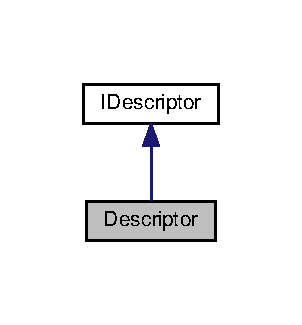
\includegraphics[width=145pt]{classDescriptor__inherit__graph}
\end{center}
\end{figure}


Collaboration diagram for Descriptor\+:
\nopagebreak
\begin{figure}[H]
\begin{center}
\leavevmode
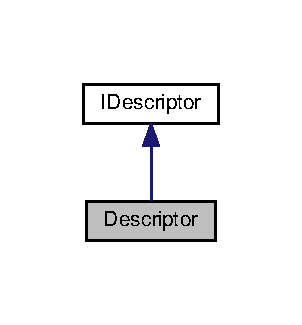
\includegraphics[width=145pt]{classDescriptor__coll__graph}
\end{center}
\end{figure}
\subsection*{Public Member Functions}
\begin{DoxyCompactItemize}
\item 
std\+::vector$<$ cv\+::\+Rect $>$ \hyperlink{classDescriptor_a86ffd0cfea1cceb0d8fae834d4cef400}{detect} (cv\+::\+Mat image)
\end{DoxyCompactItemize}
\subsection*{Private Attributes}
\begin{DoxyCompactItemize}
\item 
cv\+::\+H\+O\+G\+Descriptor \hyperlink{classDescriptor_acece8c519bd6c6de02076c405929fb9c}{descriptor}
\end{DoxyCompactItemize}


\subsection{Member Function Documentation}
\index{Descriptor@{Descriptor}!detect@{detect}}
\index{detect@{detect}!Descriptor@{Descriptor}}
\subsubsection[{\texorpdfstring{detect(cv\+::\+Mat image)}{detect(cv::Mat image)}}]{\setlength{\rightskip}{0pt plus 5cm}std\+::vector$<$ cv\+::\+Rect $>$ Descriptor\+::detect (
\begin{DoxyParamCaption}
\item[{cv\+::\+Mat}]{image}
\end{DoxyParamCaption}
)\hspace{0.3cm}{\ttfamily [virtual]}}\hypertarget{classDescriptor_a86ffd0cfea1cceb0d8fae834d4cef400}{}\label{classDescriptor_a86ffd0cfea1cceb0d8fae834d4cef400}


Implements \hyperlink{classIDescriptor_a5ad6a8f78f4799db452d7f709de36986}{I\+Descriptor}.



\subsection{Member Data Documentation}
\index{Descriptor@{Descriptor}!descriptor@{descriptor}}
\index{descriptor@{descriptor}!Descriptor@{Descriptor}}
\subsubsection[{\texorpdfstring{descriptor}{descriptor}}]{\setlength{\rightskip}{0pt plus 5cm}cv\+::\+H\+O\+G\+Descriptor Descriptor\+::descriptor\hspace{0.3cm}{\ttfamily [private]}}\hypertarget{classDescriptor_acece8c519bd6c6de02076c405929fb9c}{}\label{classDescriptor_acece8c519bd6c6de02076c405929fb9c}


The documentation for this class was generated from the following files\+:\begin{DoxyCompactItemize}
\item 
include/\hyperlink{Descriptor_8hpp}{Descriptor.\+hpp}\item 
app/\hyperlink{Descriptor_8cpp}{Descriptor.\+cpp}\end{DoxyCompactItemize}

\hypertarget{classDescriptorMock}{}\section{Descriptor\+Mock Class Reference}
\label{classDescriptorMock}\index{Descriptor\+Mock@{Descriptor\+Mock}}


{\ttfamily \#include $<$Descriptor\+Mock.\+hpp$>$}



Inheritance diagram for Descriptor\+Mock\+:
\nopagebreak
\begin{figure}[H]
\begin{center}
\leavevmode
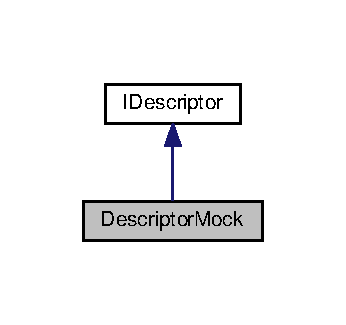
\includegraphics[width=166pt]{classDescriptorMock__inherit__graph}
\end{center}
\end{figure}


Collaboration diagram for Descriptor\+Mock\+:
\nopagebreak
\begin{figure}[H]
\begin{center}
\leavevmode
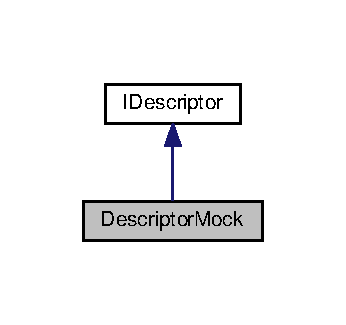
\includegraphics[width=166pt]{classDescriptorMock__coll__graph}
\end{center}
\end{figure}
\subsection*{Public Member Functions}
\begin{DoxyCompactItemize}
\item 
std\+::vector$<$ cv\+::\+Rect $>$ \hyperlink{classDescriptorMock_ae072c43f4f6621ffbd81b186e5470f38}{detect} (cv\+::\+Mat image)
\end{DoxyCompactItemize}


\subsection{Member Function Documentation}
\index{Descriptor\+Mock@{Descriptor\+Mock}!detect@{detect}}
\index{detect@{detect}!Descriptor\+Mock@{Descriptor\+Mock}}
\subsubsection[{\texorpdfstring{detect(cv\+::\+Mat image)}{detect(cv::Mat image)}}]{\setlength{\rightskip}{0pt plus 5cm}std\+::vector$<$cv\+::\+Rect$>$ Descriptor\+Mock\+::detect (
\begin{DoxyParamCaption}
\item[{cv\+::\+Mat}]{image}
\end{DoxyParamCaption}
)\hspace{0.3cm}{\ttfamily [inline]}, {\ttfamily [virtual]}}\hypertarget{classDescriptorMock_ae072c43f4f6621ffbd81b186e5470f38}{}\label{classDescriptorMock_ae072c43f4f6621ffbd81b186e5470f38}


Implements \hyperlink{classIDescriptor_a5ad6a8f78f4799db452d7f709de36986}{I\+Descriptor}.



The documentation for this class was generated from the following file\+:\begin{DoxyCompactItemize}
\item 
test/\hyperlink{DescriptorMock_8hpp}{Descriptor\+Mock.\+hpp}\end{DoxyCompactItemize}

\hypertarget{classHumanDetector}{}\section{Human\+Detector Class Reference}
\label{classHumanDetector}\index{Human\+Detector@{Human\+Detector}}


{\ttfamily \#include $<$Human\+Detector.\+hpp$>$}



Collaboration diagram for Human\+Detector\+:
\nopagebreak
\begin{figure}[H]
\begin{center}
\leavevmode
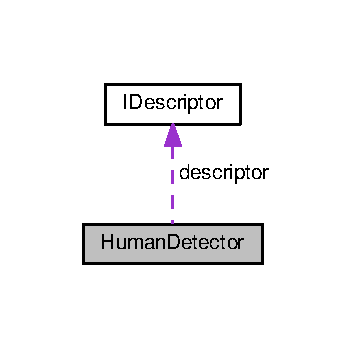
\includegraphics[width=169pt]{classHumanDetector__coll__graph}
\end{center}
\end{figure}
\subsection*{Public Member Functions}
\begin{DoxyCompactItemize}
\item 
\hyperlink{classHumanDetector_a8910bbd14716e8e47a4f3d33daeb5eba}{Human\+Detector} ()
\item 
std\+::vector$<$ cv\+::\+Rect $>$ \hyperlink{classHumanDetector_ac3c3f22f9c79dc927085f9d0bea7aeac}{detect\+Human} (cv\+::\+Mat image)
\item 
std\+::vector$<$ cv\+::\+Rect $>$ \hyperlink{classHumanDetector_aa8923db715d106cfbe4ef5f4aadc87d0}{improve\+Boundary} (std\+::vector$<$ cv\+::\+Rect $>$ \hyperlink{classHumanDetector_acbdcb52dde539827a65d86829cc90ce3}{boundary})
\item 
std\+::vector$<$ cv\+::\+Rect $>$ \hyperlink{classHumanDetector_ae5ab3f70b303e82a52b779eaedcf7709}{get\+Boundary} () const 
\item 
void \hyperlink{classHumanDetector_a02a790efcb7f2619b6ccff2195b0a95a}{set\+Boundary} (std\+::vector$<$ cv\+::\+Rect $>$ bound)
\item 
cv\+::\+Mat \hyperlink{classHumanDetector_a0faff34f61f2c60e41f8b355de2b7700}{get\+Image\+Frame} () const 
\item 
void \hyperlink{classHumanDetector_ab20928eff64db213e7e43b4a41ba6b5e}{set\+Image\+Frame} (cv\+::\+Mat \hyperlink{classHumanDetector_a5a075756a9b9ff4f0fa9fcd5fbe757b8}{image\+Frame})
\item 
\hyperlink{classIDescriptor}{I\+Descriptor} $\ast$ \hyperlink{classHumanDetector_acadd0401a44143430c329ab9393027c8}{get\+Descriptor} () const 
\item 
void \hyperlink{classHumanDetector_a2e3d5a1f08d525599b706a76926f65d5}{set\+Descriptor} (\hyperlink{classIDescriptor}{I\+Descriptor} $\ast$desc)
\end{DoxyCompactItemize}
\subsection*{Private Attributes}
\begin{DoxyCompactItemize}
\item 
\hyperlink{classIDescriptor}{I\+Descriptor} $\ast$ \hyperlink{classHumanDetector_a920f67ab988786133b5fd478a0711965}{descriptor}
\item 
std\+::vector$<$ cv\+::\+Rect $>$ \hyperlink{classHumanDetector_acbdcb52dde539827a65d86829cc90ce3}{boundary}
\item 
cv\+::\+Mat \hyperlink{classHumanDetector_a5a075756a9b9ff4f0fa9fcd5fbe757b8}{image\+Frame}
\end{DoxyCompactItemize}


\subsection{Constructor \& Destructor Documentation}
\index{Human\+Detector@{Human\+Detector}!Human\+Detector@{Human\+Detector}}
\index{Human\+Detector@{Human\+Detector}!Human\+Detector@{Human\+Detector}}
\subsubsection[{\texorpdfstring{Human\+Detector()}{HumanDetector()}}]{\setlength{\rightskip}{0pt plus 5cm}Human\+Detector\+::\+Human\+Detector (
\begin{DoxyParamCaption}
{}
\end{DoxyParamCaption}
)\hspace{0.3cm}{\ttfamily [inline]}}\hypertarget{classHumanDetector_a8910bbd14716e8e47a4f3d33daeb5eba}{}\label{classHumanDetector_a8910bbd14716e8e47a4f3d33daeb5eba}


\subsection{Member Function Documentation}
\index{Human\+Detector@{Human\+Detector}!detect\+Human@{detect\+Human}}
\index{detect\+Human@{detect\+Human}!Human\+Detector@{Human\+Detector}}
\subsubsection[{\texorpdfstring{detect\+Human(cv\+::\+Mat image)}{detectHuman(cv::Mat image)}}]{\setlength{\rightskip}{0pt plus 5cm}std\+::vector$<$ cv\+::\+Rect $>$ Human\+Detector\+::detect\+Human (
\begin{DoxyParamCaption}
\item[{cv\+::\+Mat}]{image}
\end{DoxyParamCaption}
)}\hypertarget{classHumanDetector_ac3c3f22f9c79dc927085f9d0bea7aeac}{}\label{classHumanDetector_ac3c3f22f9c79dc927085f9d0bea7aeac}
\index{Human\+Detector@{Human\+Detector}!get\+Boundary@{get\+Boundary}}
\index{get\+Boundary@{get\+Boundary}!Human\+Detector@{Human\+Detector}}
\subsubsection[{\texorpdfstring{get\+Boundary() const }{getBoundary() const }}]{\setlength{\rightskip}{0pt plus 5cm}std\+::vector$<$cv\+::\+Rect$>$ Human\+Detector\+::get\+Boundary (
\begin{DoxyParamCaption}
{}
\end{DoxyParamCaption}
) const\hspace{0.3cm}{\ttfamily [inline]}}\hypertarget{classHumanDetector_ae5ab3f70b303e82a52b779eaedcf7709}{}\label{classHumanDetector_ae5ab3f70b303e82a52b779eaedcf7709}
\index{Human\+Detector@{Human\+Detector}!get\+Descriptor@{get\+Descriptor}}
\index{get\+Descriptor@{get\+Descriptor}!Human\+Detector@{Human\+Detector}}
\subsubsection[{\texorpdfstring{get\+Descriptor() const }{getDescriptor() const }}]{\setlength{\rightskip}{0pt plus 5cm}{\bf I\+Descriptor}$\ast$ Human\+Detector\+::get\+Descriptor (
\begin{DoxyParamCaption}
{}
\end{DoxyParamCaption}
) const\hspace{0.3cm}{\ttfamily [inline]}}\hypertarget{classHumanDetector_acadd0401a44143430c329ab9393027c8}{}\label{classHumanDetector_acadd0401a44143430c329ab9393027c8}
\index{Human\+Detector@{Human\+Detector}!get\+Image\+Frame@{get\+Image\+Frame}}
\index{get\+Image\+Frame@{get\+Image\+Frame}!Human\+Detector@{Human\+Detector}}
\subsubsection[{\texorpdfstring{get\+Image\+Frame() const }{getImageFrame() const }}]{\setlength{\rightskip}{0pt plus 5cm}cv\+::\+Mat Human\+Detector\+::get\+Image\+Frame (
\begin{DoxyParamCaption}
{}
\end{DoxyParamCaption}
) const\hspace{0.3cm}{\ttfamily [inline]}}\hypertarget{classHumanDetector_a0faff34f61f2c60e41f8b355de2b7700}{}\label{classHumanDetector_a0faff34f61f2c60e41f8b355de2b7700}
\index{Human\+Detector@{Human\+Detector}!improve\+Boundary@{improve\+Boundary}}
\index{improve\+Boundary@{improve\+Boundary}!Human\+Detector@{Human\+Detector}}
\subsubsection[{\texorpdfstring{improve\+Boundary(std\+::vector$<$ cv\+::\+Rect $>$ boundary)}{improveBoundary(std::vector< cv::Rect > boundary)}}]{\setlength{\rightskip}{0pt plus 5cm}std\+::vector$<$ cv\+::\+Rect $>$ Human\+Detector\+::improve\+Boundary (
\begin{DoxyParamCaption}
\item[{std\+::vector$<$ cv\+::\+Rect $>$}]{boundary}
\end{DoxyParamCaption}
)}\hypertarget{classHumanDetector_aa8923db715d106cfbe4ef5f4aadc87d0}{}\label{classHumanDetector_aa8923db715d106cfbe4ef5f4aadc87d0}
\index{Human\+Detector@{Human\+Detector}!set\+Boundary@{set\+Boundary}}
\index{set\+Boundary@{set\+Boundary}!Human\+Detector@{Human\+Detector}}
\subsubsection[{\texorpdfstring{set\+Boundary(std\+::vector$<$ cv\+::\+Rect $>$ bound)}{setBoundary(std::vector< cv::Rect > bound)}}]{\setlength{\rightskip}{0pt plus 5cm}void Human\+Detector\+::set\+Boundary (
\begin{DoxyParamCaption}
\item[{std\+::vector$<$ cv\+::\+Rect $>$}]{bound}
\end{DoxyParamCaption}
)\hspace{0.3cm}{\ttfamily [inline]}}\hypertarget{classHumanDetector_a02a790efcb7f2619b6ccff2195b0a95a}{}\label{classHumanDetector_a02a790efcb7f2619b6ccff2195b0a95a}
\index{Human\+Detector@{Human\+Detector}!set\+Descriptor@{set\+Descriptor}}
\index{set\+Descriptor@{set\+Descriptor}!Human\+Detector@{Human\+Detector}}
\subsubsection[{\texorpdfstring{set\+Descriptor(\+I\+Descriptor $\ast$desc)}{setDescriptor(IDescriptor *desc)}}]{\setlength{\rightskip}{0pt plus 5cm}void Human\+Detector\+::set\+Descriptor (
\begin{DoxyParamCaption}
\item[{{\bf I\+Descriptor} $\ast$}]{desc}
\end{DoxyParamCaption}
)\hspace{0.3cm}{\ttfamily [inline]}}\hypertarget{classHumanDetector_a2e3d5a1f08d525599b706a76926f65d5}{}\label{classHumanDetector_a2e3d5a1f08d525599b706a76926f65d5}
\index{Human\+Detector@{Human\+Detector}!set\+Image\+Frame@{set\+Image\+Frame}}
\index{set\+Image\+Frame@{set\+Image\+Frame}!Human\+Detector@{Human\+Detector}}
\subsubsection[{\texorpdfstring{set\+Image\+Frame(cv\+::\+Mat image\+Frame)}{setImageFrame(cv::Mat imageFrame)}}]{\setlength{\rightskip}{0pt plus 5cm}void Human\+Detector\+::set\+Image\+Frame (
\begin{DoxyParamCaption}
\item[{cv\+::\+Mat}]{image\+Frame}
\end{DoxyParamCaption}
)\hspace{0.3cm}{\ttfamily [inline]}}\hypertarget{classHumanDetector_ab20928eff64db213e7e43b4a41ba6b5e}{}\label{classHumanDetector_ab20928eff64db213e7e43b4a41ba6b5e}


\subsection{Member Data Documentation}
\index{Human\+Detector@{Human\+Detector}!boundary@{boundary}}
\index{boundary@{boundary}!Human\+Detector@{Human\+Detector}}
\subsubsection[{\texorpdfstring{boundary}{boundary}}]{\setlength{\rightskip}{0pt plus 5cm}std\+::vector$<$cv\+::\+Rect$>$ Human\+Detector\+::boundary\hspace{0.3cm}{\ttfamily [private]}}\hypertarget{classHumanDetector_acbdcb52dde539827a65d86829cc90ce3}{}\label{classHumanDetector_acbdcb52dde539827a65d86829cc90ce3}
\index{Human\+Detector@{Human\+Detector}!descriptor@{descriptor}}
\index{descriptor@{descriptor}!Human\+Detector@{Human\+Detector}}
\subsubsection[{\texorpdfstring{descriptor}{descriptor}}]{\setlength{\rightskip}{0pt plus 5cm}{\bf I\+Descriptor}$\ast$ Human\+Detector\+::descriptor\hspace{0.3cm}{\ttfamily [private]}}\hypertarget{classHumanDetector_a920f67ab988786133b5fd478a0711965}{}\label{classHumanDetector_a920f67ab988786133b5fd478a0711965}
\index{Human\+Detector@{Human\+Detector}!image\+Frame@{image\+Frame}}
\index{image\+Frame@{image\+Frame}!Human\+Detector@{Human\+Detector}}
\subsubsection[{\texorpdfstring{image\+Frame}{imageFrame}}]{\setlength{\rightskip}{0pt plus 5cm}cv\+::\+Mat Human\+Detector\+::image\+Frame\hspace{0.3cm}{\ttfamily [private]}}\hypertarget{classHumanDetector_a5a075756a9b9ff4f0fa9fcd5fbe757b8}{}\label{classHumanDetector_a5a075756a9b9ff4f0fa9fcd5fbe757b8}


The documentation for this class was generated from the following files\+:\begin{DoxyCompactItemize}
\item 
include/\hyperlink{HumanDetector_8hpp}{Human\+Detector.\+hpp}\item 
app/\hyperlink{HumanDetector_8cpp}{Human\+Detector.\+cpp}\end{DoxyCompactItemize}

\hypertarget{classIDescriptor}{}\section{I\+Descriptor Class Reference}
\label{classIDescriptor}\index{I\+Descriptor@{I\+Descriptor}}


{\ttfamily \#include $<$I\+Descriptor.\+hpp$>$}



Inheritance diagram for I\+Descriptor\+:
\nopagebreak
\begin{figure}[H]
\begin{center}
\leavevmode
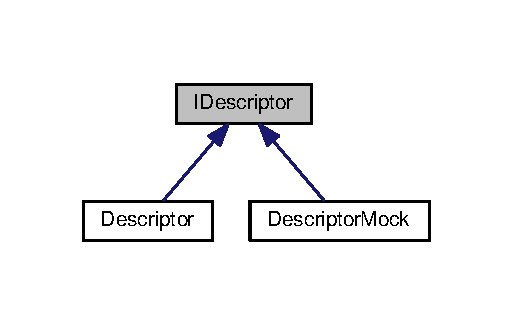
\includegraphics[width=246pt]{classIDescriptor__inherit__graph}
\end{center}
\end{figure}
\subsection*{Public Member Functions}
\begin{DoxyCompactItemize}
\item 
virtual std\+::vector$<$ cv\+::\+Rect $>$ \hyperlink{classIDescriptor_a5ad6a8f78f4799db452d7f709de36986}{detect} (cv\+::\+Mat image)=0
\end{DoxyCompactItemize}


\subsection{Member Function Documentation}
\index{I\+Descriptor@{I\+Descriptor}!detect@{detect}}
\index{detect@{detect}!I\+Descriptor@{I\+Descriptor}}
\subsubsection[{\texorpdfstring{detect(cv\+::\+Mat image)=0}{detect(cv::Mat image)=0}}]{\setlength{\rightskip}{0pt plus 5cm}virtual std\+::vector$<$cv\+::\+Rect$>$ I\+Descriptor\+::detect (
\begin{DoxyParamCaption}
\item[{cv\+::\+Mat}]{image}
\end{DoxyParamCaption}
)\hspace{0.3cm}{\ttfamily [pure virtual]}}\hypertarget{classIDescriptor_a5ad6a8f78f4799db452d7f709de36986}{}\label{classIDescriptor_a5ad6a8f78f4799db452d7f709de36986}


Implemented in \hyperlink{classDescriptor_a86ffd0cfea1cceb0d8fae834d4cef400}{Descriptor}, and \hyperlink{classDescriptorMock_ae072c43f4f6621ffbd81b186e5470f38}{Descriptor\+Mock}.



The documentation for this class was generated from the following file\+:\begin{DoxyCompactItemize}
\item 
include/\hyperlink{IDescriptor_8hpp}{I\+Descriptor.\+hpp}\end{DoxyCompactItemize}

\hypertarget{classImageInput}{}\section{Image\+Input Class Reference}
\label{classImageInput}\index{Image\+Input@{Image\+Input}}


{\ttfamily \#include $<$Image\+Input.\+hpp$>$}



Collaboration diagram for Image\+Input\+:
\nopagebreak
\begin{figure}[H]
\begin{center}
\leavevmode
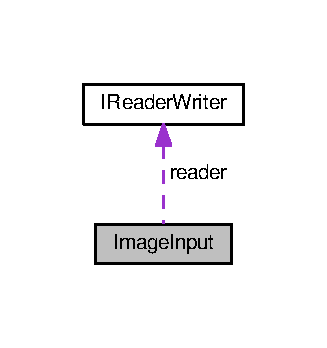
\includegraphics[width=157pt]{classImageInput__coll__graph}
\end{center}
\end{figure}
\subsection*{Public Member Functions}
\begin{DoxyCompactItemize}
\item 
\hyperlink{classImageInput_aca508a0b68659c71ad378cc0f2250298}{Image\+Input} ()
\item 
cv\+::\+Mat \hyperlink{classImageInput_a900eac6479654160858d9fe344bbf6d6}{read\+Image} (std\+::string image\+Path)
\item 
cv\+::\+Mat \hyperlink{classImageInput_a084f7e45ebe22d2ebbb507e7e1886988}{get\+Image\+Frame} () const 
\item 
void \hyperlink{classImageInput_ab2b3f3771c15d7172c4cd10dcb0d573e}{set\+Image\+Frame} (cv\+::\+Mat \hyperlink{classImageInput_a94723568a2a817760fe4e38fc11efb25}{image\+Frame})
\item 
\hyperlink{classIReaderWriter}{I\+Reader\+Writer} $\ast$ \hyperlink{classImageInput_a4b49b8a4ec9713412416ebd6de3753de}{get\+Reader} () const 
\item 
void \hyperlink{classImageInput_af61cc921f9911bef3d749fbc87ddf811}{set\+Reader} (\hyperlink{classIReaderWriter}{I\+Reader\+Writer} $\ast$r)
\end{DoxyCompactItemize}
\subsection*{Private Attributes}
\begin{DoxyCompactItemize}
\item 
cv\+::\+Mat \hyperlink{classImageInput_a94723568a2a817760fe4e38fc11efb25}{image\+Frame}
\item 
\hyperlink{classIReaderWriter}{I\+Reader\+Writer} $\ast$ \hyperlink{classImageInput_a23a93c13b57550831c58c0b5485efe01}{reader}
\end{DoxyCompactItemize}


\subsection{Constructor \& Destructor Documentation}
\index{Image\+Input@{Image\+Input}!Image\+Input@{Image\+Input}}
\index{Image\+Input@{Image\+Input}!Image\+Input@{Image\+Input}}
\subsubsection[{\texorpdfstring{Image\+Input()}{ImageInput()}}]{\setlength{\rightskip}{0pt plus 5cm}Image\+Input\+::\+Image\+Input (
\begin{DoxyParamCaption}
{}
\end{DoxyParamCaption}
)\hspace{0.3cm}{\ttfamily [inline]}}\hypertarget{classImageInput_aca508a0b68659c71ad378cc0f2250298}{}\label{classImageInput_aca508a0b68659c71ad378cc0f2250298}


\subsection{Member Function Documentation}
\index{Image\+Input@{Image\+Input}!get\+Image\+Frame@{get\+Image\+Frame}}
\index{get\+Image\+Frame@{get\+Image\+Frame}!Image\+Input@{Image\+Input}}
\subsubsection[{\texorpdfstring{get\+Image\+Frame() const }{getImageFrame() const }}]{\setlength{\rightskip}{0pt plus 5cm}cv\+::\+Mat Image\+Input\+::get\+Image\+Frame (
\begin{DoxyParamCaption}
{}
\end{DoxyParamCaption}
) const\hspace{0.3cm}{\ttfamily [inline]}}\hypertarget{classImageInput_a084f7e45ebe22d2ebbb507e7e1886988}{}\label{classImageInput_a084f7e45ebe22d2ebbb507e7e1886988}
\index{Image\+Input@{Image\+Input}!get\+Reader@{get\+Reader}}
\index{get\+Reader@{get\+Reader}!Image\+Input@{Image\+Input}}
\subsubsection[{\texorpdfstring{get\+Reader() const }{getReader() const }}]{\setlength{\rightskip}{0pt plus 5cm}{\bf I\+Reader\+Writer}$\ast$ Image\+Input\+::get\+Reader (
\begin{DoxyParamCaption}
{}
\end{DoxyParamCaption}
) const\hspace{0.3cm}{\ttfamily [inline]}}\hypertarget{classImageInput_a4b49b8a4ec9713412416ebd6de3753de}{}\label{classImageInput_a4b49b8a4ec9713412416ebd6de3753de}
\index{Image\+Input@{Image\+Input}!read\+Image@{read\+Image}}
\index{read\+Image@{read\+Image}!Image\+Input@{Image\+Input}}
\subsubsection[{\texorpdfstring{read\+Image(std\+::string image\+Path)}{readImage(std::string imagePath)}}]{\setlength{\rightskip}{0pt plus 5cm}cv\+::\+Mat Image\+Input\+::read\+Image (
\begin{DoxyParamCaption}
\item[{std\+::string}]{image\+Path}
\end{DoxyParamCaption}
)}\hypertarget{classImageInput_a900eac6479654160858d9fe344bbf6d6}{}\label{classImageInput_a900eac6479654160858d9fe344bbf6d6}
\index{Image\+Input@{Image\+Input}!set\+Image\+Frame@{set\+Image\+Frame}}
\index{set\+Image\+Frame@{set\+Image\+Frame}!Image\+Input@{Image\+Input}}
\subsubsection[{\texorpdfstring{set\+Image\+Frame(cv\+::\+Mat image\+Frame)}{setImageFrame(cv::Mat imageFrame)}}]{\setlength{\rightskip}{0pt plus 5cm}void Image\+Input\+::set\+Image\+Frame (
\begin{DoxyParamCaption}
\item[{cv\+::\+Mat}]{image\+Frame}
\end{DoxyParamCaption}
)\hspace{0.3cm}{\ttfamily [inline]}}\hypertarget{classImageInput_ab2b3f3771c15d7172c4cd10dcb0d573e}{}\label{classImageInput_ab2b3f3771c15d7172c4cd10dcb0d573e}
\index{Image\+Input@{Image\+Input}!set\+Reader@{set\+Reader}}
\index{set\+Reader@{set\+Reader}!Image\+Input@{Image\+Input}}
\subsubsection[{\texorpdfstring{set\+Reader(\+I\+Reader\+Writer $\ast$r)}{setReader(IReaderWriter *r)}}]{\setlength{\rightskip}{0pt plus 5cm}void Image\+Input\+::set\+Reader (
\begin{DoxyParamCaption}
\item[{{\bf I\+Reader\+Writer} $\ast$}]{r}
\end{DoxyParamCaption}
)\hspace{0.3cm}{\ttfamily [inline]}}\hypertarget{classImageInput_af61cc921f9911bef3d749fbc87ddf811}{}\label{classImageInput_af61cc921f9911bef3d749fbc87ddf811}


\subsection{Member Data Documentation}
\index{Image\+Input@{Image\+Input}!image\+Frame@{image\+Frame}}
\index{image\+Frame@{image\+Frame}!Image\+Input@{Image\+Input}}
\subsubsection[{\texorpdfstring{image\+Frame}{imageFrame}}]{\setlength{\rightskip}{0pt plus 5cm}cv\+::\+Mat Image\+Input\+::image\+Frame\hspace{0.3cm}{\ttfamily [private]}}\hypertarget{classImageInput_a94723568a2a817760fe4e38fc11efb25}{}\label{classImageInput_a94723568a2a817760fe4e38fc11efb25}
\index{Image\+Input@{Image\+Input}!reader@{reader}}
\index{reader@{reader}!Image\+Input@{Image\+Input}}
\subsubsection[{\texorpdfstring{reader}{reader}}]{\setlength{\rightskip}{0pt plus 5cm}{\bf I\+Reader\+Writer}$\ast$ Image\+Input\+::reader\hspace{0.3cm}{\ttfamily [private]}}\hypertarget{classImageInput_a23a93c13b57550831c58c0b5485efe01}{}\label{classImageInput_a23a93c13b57550831c58c0b5485efe01}


The documentation for this class was generated from the following files\+:\begin{DoxyCompactItemize}
\item 
include/\hyperlink{ImageInput_8hpp}{Image\+Input.\+hpp}\item 
app/\hyperlink{ImageInput_8cpp}{Image\+Input.\+cpp}\end{DoxyCompactItemize}

\hypertarget{classImageOutput}{}\section{Image\+Output Class Reference}
\label{classImageOutput}\index{Image\+Output@{Image\+Output}}


{\ttfamily \#include $<$Image\+Output.\+hpp$>$}



Collaboration diagram for Image\+Output\+:
\nopagebreak
\begin{figure}[H]
\begin{center}
\leavevmode
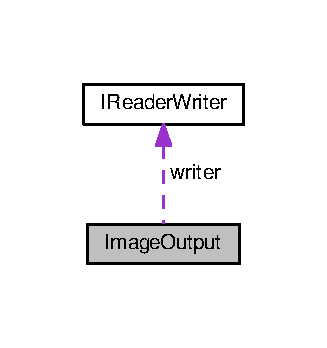
\includegraphics[width=157pt]{classImageOutput__coll__graph}
\end{center}
\end{figure}
\subsection*{Public Member Functions}
\begin{DoxyCompactItemize}
\item 
\hyperlink{classImageOutput_acd191c0743501f00240fa87080db187d}{Image\+Output} ()
\item 
void \hyperlink{classImageOutput_a366b4b4dc1a3d42b4c6dd2601a5668c6}{show\+Image} (cv\+::\+Mat image)
\item 
cv\+::\+Mat \hyperlink{classImageOutput_af2d882c564dc495b263a9c7dfdde2671}{draw\+Boundary} (cv\+::\+Mat image, std\+::vector$<$ cv\+::\+Rect $>$ \hyperlink{classImageOutput_acf9d0f7617433a905fcd5deeed24ed65}{boundary})
\item 
std\+::vector$<$ cv\+::\+Rect $>$ \hyperlink{classImageOutput_a9bd38d9812c4c70fd646ce569d183469}{get\+Boundary} () const 
\item 
void \hyperlink{classImageOutput_a79f7ae3fb3091629232f9b04a3b3232e}{set\+Boundary} (std\+::vector$<$ cv\+::\+Rect $>$ bound)
\item 
\hyperlink{classIReaderWriter}{I\+Reader\+Writer} $\ast$ \hyperlink{classImageOutput_a7d673d591761131af199d8284c7ebbe5}{get\+Writer} () const 
\item 
void \hyperlink{classImageOutput_abd982398c9a8ce648119f3088964014f}{set\+Writer} (\hyperlink{classIReaderWriter}{I\+Reader\+Writer} $\ast$w)
\end{DoxyCompactItemize}
\subsection*{Private Attributes}
\begin{DoxyCompactItemize}
\item 
std\+::vector$<$ cv\+::\+Rect $>$ \hyperlink{classImageOutput_acf9d0f7617433a905fcd5deeed24ed65}{boundary}
\item 
\hyperlink{classIReaderWriter}{I\+Reader\+Writer} $\ast$ \hyperlink{classImageOutput_a830504828d51af19fe99c1663c01b4c6}{writer}
\end{DoxyCompactItemize}


\subsection{Constructor \& Destructor Documentation}
\index{Image\+Output@{Image\+Output}!Image\+Output@{Image\+Output}}
\index{Image\+Output@{Image\+Output}!Image\+Output@{Image\+Output}}
\subsubsection[{\texorpdfstring{Image\+Output()}{ImageOutput()}}]{\setlength{\rightskip}{0pt plus 5cm}Image\+Output\+::\+Image\+Output (
\begin{DoxyParamCaption}
{}
\end{DoxyParamCaption}
)\hspace{0.3cm}{\ttfamily [inline]}}\hypertarget{classImageOutput_acd191c0743501f00240fa87080db187d}{}\label{classImageOutput_acd191c0743501f00240fa87080db187d}


\subsection{Member Function Documentation}
\index{Image\+Output@{Image\+Output}!draw\+Boundary@{draw\+Boundary}}
\index{draw\+Boundary@{draw\+Boundary}!Image\+Output@{Image\+Output}}
\subsubsection[{\texorpdfstring{draw\+Boundary(cv\+::\+Mat image, std\+::vector$<$ cv\+::\+Rect $>$ boundary)}{drawBoundary(cv::Mat image, std::vector< cv::Rect > boundary)}}]{\setlength{\rightskip}{0pt plus 5cm}cv\+::\+Mat Image\+Output\+::draw\+Boundary (
\begin{DoxyParamCaption}
\item[{cv\+::\+Mat}]{image, }
\item[{std\+::vector$<$ cv\+::\+Rect $>$}]{boundary}
\end{DoxyParamCaption}
)}\hypertarget{classImageOutput_af2d882c564dc495b263a9c7dfdde2671}{}\label{classImageOutput_af2d882c564dc495b263a9c7dfdde2671}
\index{Image\+Output@{Image\+Output}!get\+Boundary@{get\+Boundary}}
\index{get\+Boundary@{get\+Boundary}!Image\+Output@{Image\+Output}}
\subsubsection[{\texorpdfstring{get\+Boundary() const }{getBoundary() const }}]{\setlength{\rightskip}{0pt plus 5cm}std\+::vector$<$cv\+::\+Rect$>$ Image\+Output\+::get\+Boundary (
\begin{DoxyParamCaption}
{}
\end{DoxyParamCaption}
) const\hspace{0.3cm}{\ttfamily [inline]}}\hypertarget{classImageOutput_a9bd38d9812c4c70fd646ce569d183469}{}\label{classImageOutput_a9bd38d9812c4c70fd646ce569d183469}
\index{Image\+Output@{Image\+Output}!get\+Writer@{get\+Writer}}
\index{get\+Writer@{get\+Writer}!Image\+Output@{Image\+Output}}
\subsubsection[{\texorpdfstring{get\+Writer() const }{getWriter() const }}]{\setlength{\rightskip}{0pt plus 5cm}{\bf I\+Reader\+Writer}$\ast$ Image\+Output\+::get\+Writer (
\begin{DoxyParamCaption}
{}
\end{DoxyParamCaption}
) const\hspace{0.3cm}{\ttfamily [inline]}}\hypertarget{classImageOutput_a7d673d591761131af199d8284c7ebbe5}{}\label{classImageOutput_a7d673d591761131af199d8284c7ebbe5}
\index{Image\+Output@{Image\+Output}!set\+Boundary@{set\+Boundary}}
\index{set\+Boundary@{set\+Boundary}!Image\+Output@{Image\+Output}}
\subsubsection[{\texorpdfstring{set\+Boundary(std\+::vector$<$ cv\+::\+Rect $>$ bound)}{setBoundary(std::vector< cv::Rect > bound)}}]{\setlength{\rightskip}{0pt plus 5cm}void Image\+Output\+::set\+Boundary (
\begin{DoxyParamCaption}
\item[{std\+::vector$<$ cv\+::\+Rect $>$}]{bound}
\end{DoxyParamCaption}
)\hspace{0.3cm}{\ttfamily [inline]}}\hypertarget{classImageOutput_a79f7ae3fb3091629232f9b04a3b3232e}{}\label{classImageOutput_a79f7ae3fb3091629232f9b04a3b3232e}
\index{Image\+Output@{Image\+Output}!set\+Writer@{set\+Writer}}
\index{set\+Writer@{set\+Writer}!Image\+Output@{Image\+Output}}
\subsubsection[{\texorpdfstring{set\+Writer(\+I\+Reader\+Writer $\ast$w)}{setWriter(IReaderWriter *w)}}]{\setlength{\rightskip}{0pt plus 5cm}void Image\+Output\+::set\+Writer (
\begin{DoxyParamCaption}
\item[{{\bf I\+Reader\+Writer} $\ast$}]{w}
\end{DoxyParamCaption}
)\hspace{0.3cm}{\ttfamily [inline]}}\hypertarget{classImageOutput_abd982398c9a8ce648119f3088964014f}{}\label{classImageOutput_abd982398c9a8ce648119f3088964014f}
\index{Image\+Output@{Image\+Output}!show\+Image@{show\+Image}}
\index{show\+Image@{show\+Image}!Image\+Output@{Image\+Output}}
\subsubsection[{\texorpdfstring{show\+Image(cv\+::\+Mat image)}{showImage(cv::Mat image)}}]{\setlength{\rightskip}{0pt plus 5cm}void Image\+Output\+::show\+Image (
\begin{DoxyParamCaption}
\item[{cv\+::\+Mat}]{image}
\end{DoxyParamCaption}
)}\hypertarget{classImageOutput_a366b4b4dc1a3d42b4c6dd2601a5668c6}{}\label{classImageOutput_a366b4b4dc1a3d42b4c6dd2601a5668c6}


\subsection{Member Data Documentation}
\index{Image\+Output@{Image\+Output}!boundary@{boundary}}
\index{boundary@{boundary}!Image\+Output@{Image\+Output}}
\subsubsection[{\texorpdfstring{boundary}{boundary}}]{\setlength{\rightskip}{0pt plus 5cm}std\+::vector$<$cv\+::\+Rect$>$ Image\+Output\+::boundary\hspace{0.3cm}{\ttfamily [private]}}\hypertarget{classImageOutput_acf9d0f7617433a905fcd5deeed24ed65}{}\label{classImageOutput_acf9d0f7617433a905fcd5deeed24ed65}
\index{Image\+Output@{Image\+Output}!writer@{writer}}
\index{writer@{writer}!Image\+Output@{Image\+Output}}
\subsubsection[{\texorpdfstring{writer}{writer}}]{\setlength{\rightskip}{0pt plus 5cm}{\bf I\+Reader\+Writer}$\ast$ Image\+Output\+::writer\hspace{0.3cm}{\ttfamily [private]}}\hypertarget{classImageOutput_a830504828d51af19fe99c1663c01b4c6}{}\label{classImageOutput_a830504828d51af19fe99c1663c01b4c6}


The documentation for this class was generated from the following files\+:\begin{DoxyCompactItemize}
\item 
include/\hyperlink{ImageOutput_8hpp}{Image\+Output.\+hpp}\item 
app/\hyperlink{ImageOutput_8cpp}{Image\+Output.\+cpp}\end{DoxyCompactItemize}

\hypertarget{classIReaderWriter}{}\section{I\+Reader\+Writer Class Reference}
\label{classIReaderWriter}\index{I\+Reader\+Writer@{I\+Reader\+Writer}}


{\ttfamily \#include $<$I\+Reader\+Writer.\+hpp$>$}



Inheritance diagram for I\+Reader\+Writer\+:
\nopagebreak
\begin{figure}[H]
\begin{center}
\leavevmode
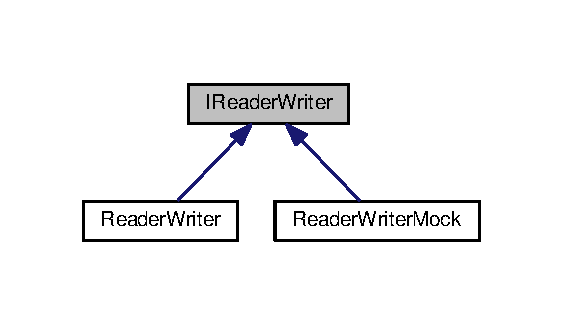
\includegraphics[width=270pt]{classIReaderWriter__inherit__graph}
\end{center}
\end{figure}
\subsection*{Public Member Functions}
\begin{DoxyCompactItemize}
\item 
virtual cv\+::\+Mat \hyperlink{classIReaderWriter_a60283bb40f3f57c55c0e7c10f320d327}{read} (std\+::string image\+Path)=0
\item 
virtual cv\+::\+Mat \hyperlink{classIReaderWriter_a59a6a668de4b600a073772c41d6d83f4}{draw\+Rectangle} (cv\+::\+Mat image, cv\+::\+Rect boundary)=0
\item 
virtual void \hyperlink{classIReaderWriter_a276d9be9746ac48b1cb0e11fb6169d90}{show\+Image} (cv\+::\+Mat image)=0
\end{DoxyCompactItemize}


\subsection{Member Function Documentation}
\index{I\+Reader\+Writer@{I\+Reader\+Writer}!draw\+Rectangle@{draw\+Rectangle}}
\index{draw\+Rectangle@{draw\+Rectangle}!I\+Reader\+Writer@{I\+Reader\+Writer}}
\subsubsection[{\texorpdfstring{draw\+Rectangle(cv\+::\+Mat image, cv\+::\+Rect boundary)=0}{drawRectangle(cv::Mat image, cv::Rect boundary)=0}}]{\setlength{\rightskip}{0pt plus 5cm}virtual cv\+::\+Mat I\+Reader\+Writer\+::draw\+Rectangle (
\begin{DoxyParamCaption}
\item[{cv\+::\+Mat}]{image, }
\item[{cv\+::\+Rect}]{boundary}
\end{DoxyParamCaption}
)\hspace{0.3cm}{\ttfamily [pure virtual]}}\hypertarget{classIReaderWriter_a59a6a668de4b600a073772c41d6d83f4}{}\label{classIReaderWriter_a59a6a668de4b600a073772c41d6d83f4}


Implemented in \hyperlink{classReaderWriter_acc7a9c2ceafa7c24983eb4f496f75d38}{Reader\+Writer}, and \hyperlink{classReaderWriterMock_a6ca66a1ca22bc7e5d18778b957f0882d}{Reader\+Writer\+Mock}.

\index{I\+Reader\+Writer@{I\+Reader\+Writer}!read@{read}}
\index{read@{read}!I\+Reader\+Writer@{I\+Reader\+Writer}}
\subsubsection[{\texorpdfstring{read(std\+::string image\+Path)=0}{read(std::string imagePath)=0}}]{\setlength{\rightskip}{0pt plus 5cm}virtual cv\+::\+Mat I\+Reader\+Writer\+::read (
\begin{DoxyParamCaption}
\item[{std\+::string}]{image\+Path}
\end{DoxyParamCaption}
)\hspace{0.3cm}{\ttfamily [pure virtual]}}\hypertarget{classIReaderWriter_a60283bb40f3f57c55c0e7c10f320d327}{}\label{classIReaderWriter_a60283bb40f3f57c55c0e7c10f320d327}


Implemented in \hyperlink{classReaderWriter_af0dd72398444d8e310ac1961d6df21e9}{Reader\+Writer}, and \hyperlink{classReaderWriterMock_a507d65810157f66de3327d6fdc58014a}{Reader\+Writer\+Mock}.

\index{I\+Reader\+Writer@{I\+Reader\+Writer}!show\+Image@{show\+Image}}
\index{show\+Image@{show\+Image}!I\+Reader\+Writer@{I\+Reader\+Writer}}
\subsubsection[{\texorpdfstring{show\+Image(cv\+::\+Mat image)=0}{showImage(cv::Mat image)=0}}]{\setlength{\rightskip}{0pt plus 5cm}virtual void I\+Reader\+Writer\+::show\+Image (
\begin{DoxyParamCaption}
\item[{cv\+::\+Mat}]{image}
\end{DoxyParamCaption}
)\hspace{0.3cm}{\ttfamily [pure virtual]}}\hypertarget{classIReaderWriter_a276d9be9746ac48b1cb0e11fb6169d90}{}\label{classIReaderWriter_a276d9be9746ac48b1cb0e11fb6169d90}


Implemented in \hyperlink{classReaderWriter_a1d17c18f4382dca87d7b54ac1c5f1828}{Reader\+Writer}, and \hyperlink{classReaderWriterMock_ab89cb39947631ebc1b5cd4b8e53650fe}{Reader\+Writer\+Mock}.



The documentation for this class was generated from the following file\+:\begin{DoxyCompactItemize}
\item 
include/\hyperlink{IReaderWriter_8hpp}{I\+Reader\+Writer.\+hpp}\end{DoxyCompactItemize}

\hypertarget{classReaderWriter}{}\section{Reader\+Writer Class Reference}
\label{classReaderWriter}\index{Reader\+Writer@{Reader\+Writer}}


{\ttfamily \#include $<$Reader\+Writer.\+hpp$>$}



Inheritance diagram for Reader\+Writer\+:
\nopagebreak
\begin{figure}[H]
\begin{center}
\leavevmode
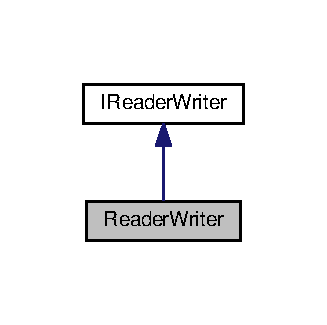
\includegraphics[width=157pt]{classReaderWriter__inherit__graph}
\end{center}
\end{figure}


Collaboration diagram for Reader\+Writer\+:
\nopagebreak
\begin{figure}[H]
\begin{center}
\leavevmode
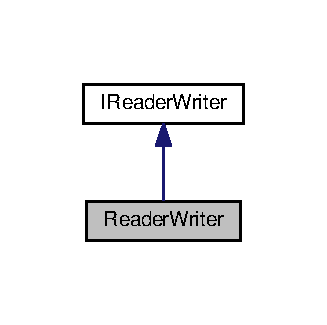
\includegraphics[width=157pt]{classReaderWriter__coll__graph}
\end{center}
\end{figure}
\subsection*{Public Member Functions}
\begin{DoxyCompactItemize}
\item 
cv\+::\+Mat \hyperlink{classReaderWriter_af0dd72398444d8e310ac1961d6df21e9}{read} (std\+::string image\+Path)
\item 
cv\+::\+Mat \hyperlink{classReaderWriter_acc7a9c2ceafa7c24983eb4f496f75d38}{draw\+Rectangle} (cv\+::\+Mat image, cv\+::\+Rect boundary)
\item 
void \hyperlink{classReaderWriter_a1d17c18f4382dca87d7b54ac1c5f1828}{show\+Image} (cv\+::\+Mat image)
\end{DoxyCompactItemize}


\subsection{Member Function Documentation}
\index{Reader\+Writer@{Reader\+Writer}!draw\+Rectangle@{draw\+Rectangle}}
\index{draw\+Rectangle@{draw\+Rectangle}!Reader\+Writer@{Reader\+Writer}}
\subsubsection[{\texorpdfstring{draw\+Rectangle(cv\+::\+Mat image, cv\+::\+Rect boundary)}{drawRectangle(cv::Mat image, cv::Rect boundary)}}]{\setlength{\rightskip}{0pt plus 5cm}cv\+::\+Mat Reader\+Writer\+::draw\+Rectangle (
\begin{DoxyParamCaption}
\item[{cv\+::\+Mat}]{image, }
\item[{cv\+::\+Rect}]{boundary}
\end{DoxyParamCaption}
)\hspace{0.3cm}{\ttfamily [virtual]}}\hypertarget{classReaderWriter_acc7a9c2ceafa7c24983eb4f496f75d38}{}\label{classReaderWriter_acc7a9c2ceafa7c24983eb4f496f75d38}


Implements \hyperlink{classIReaderWriter_a59a6a668de4b600a073772c41d6d83f4}{I\+Reader\+Writer}.

\index{Reader\+Writer@{Reader\+Writer}!read@{read}}
\index{read@{read}!Reader\+Writer@{Reader\+Writer}}
\subsubsection[{\texorpdfstring{read(std\+::string image\+Path)}{read(std::string imagePath)}}]{\setlength{\rightskip}{0pt plus 5cm}cv\+::\+Mat Reader\+Writer\+::read (
\begin{DoxyParamCaption}
\item[{std\+::string}]{image\+Path}
\end{DoxyParamCaption}
)\hspace{0.3cm}{\ttfamily [virtual]}}\hypertarget{classReaderWriter_af0dd72398444d8e310ac1961d6df21e9}{}\label{classReaderWriter_af0dd72398444d8e310ac1961d6df21e9}


Implements \hyperlink{classIReaderWriter_a60283bb40f3f57c55c0e7c10f320d327}{I\+Reader\+Writer}.

\index{Reader\+Writer@{Reader\+Writer}!show\+Image@{show\+Image}}
\index{show\+Image@{show\+Image}!Reader\+Writer@{Reader\+Writer}}
\subsubsection[{\texorpdfstring{show\+Image(cv\+::\+Mat image)}{showImage(cv::Mat image)}}]{\setlength{\rightskip}{0pt plus 5cm}void Reader\+Writer\+::show\+Image (
\begin{DoxyParamCaption}
\item[{cv\+::\+Mat}]{image}
\end{DoxyParamCaption}
)\hspace{0.3cm}{\ttfamily [virtual]}}\hypertarget{classReaderWriter_a1d17c18f4382dca87d7b54ac1c5f1828}{}\label{classReaderWriter_a1d17c18f4382dca87d7b54ac1c5f1828}


Implements \hyperlink{classIReaderWriter_a276d9be9746ac48b1cb0e11fb6169d90}{I\+Reader\+Writer}.



The documentation for this class was generated from the following files\+:\begin{DoxyCompactItemize}
\item 
include/\hyperlink{ReaderWriter_8hpp}{Reader\+Writer.\+hpp}\item 
app/\hyperlink{ReaderWriter_8cpp}{Reader\+Writer.\+cpp}\end{DoxyCompactItemize}

\hypertarget{classReaderWriterMock}{}\section{Reader\+Writer\+Mock Class Reference}
\label{classReaderWriterMock}\index{Reader\+Writer\+Mock@{Reader\+Writer\+Mock}}


{\ttfamily \#include $<$Reader\+Writer\+Mock.\+hpp$>$}



Inheritance diagram for Reader\+Writer\+Mock\+:
\nopagebreak
\begin{figure}[H]
\begin{center}
\leavevmode
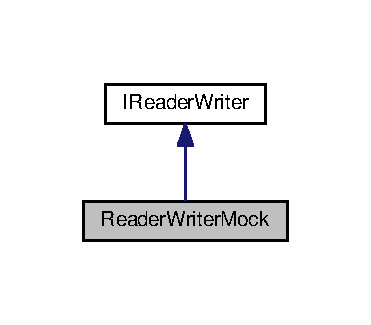
\includegraphics[width=178pt]{classReaderWriterMock__inherit__graph}
\end{center}
\end{figure}


Collaboration diagram for Reader\+Writer\+Mock\+:
\nopagebreak
\begin{figure}[H]
\begin{center}
\leavevmode
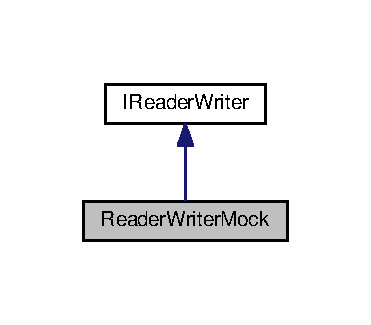
\includegraphics[width=178pt]{classReaderWriterMock__coll__graph}
\end{center}
\end{figure}
\subsection*{Public Member Functions}
\begin{DoxyCompactItemize}
\item 
cv\+::\+Mat \hyperlink{classReaderWriterMock_a507d65810157f66de3327d6fdc58014a}{read} (std\+::string image\+Path)
\item 
cv\+::\+Mat \hyperlink{classReaderWriterMock_a6ca66a1ca22bc7e5d18778b957f0882d}{draw\+Rectangle} (cv\+::\+Mat image, cv\+::\+Rect boundary)
\item 
void \hyperlink{classReaderWriterMock_ab89cb39947631ebc1b5cd4b8e53650fe}{show\+Image} (cv\+::\+Mat)
\item 
bool \hyperlink{classReaderWriterMock_aa50f28fa732ea87e1f444291bc780bef}{is\+\_\+file\+\_\+exist} (const std\+::string file\+Name)
\end{DoxyCompactItemize}


\subsection{Member Function Documentation}
\index{Reader\+Writer\+Mock@{Reader\+Writer\+Mock}!draw\+Rectangle@{draw\+Rectangle}}
\index{draw\+Rectangle@{draw\+Rectangle}!Reader\+Writer\+Mock@{Reader\+Writer\+Mock}}
\subsubsection[{\texorpdfstring{draw\+Rectangle(cv\+::\+Mat image, cv\+::\+Rect boundary)}{drawRectangle(cv::Mat image, cv::Rect boundary)}}]{\setlength{\rightskip}{0pt plus 5cm}cv\+::\+Mat Reader\+Writer\+Mock\+::draw\+Rectangle (
\begin{DoxyParamCaption}
\item[{cv\+::\+Mat}]{image, }
\item[{cv\+::\+Rect}]{boundary}
\end{DoxyParamCaption}
)\hspace{0.3cm}{\ttfamily [inline]}, {\ttfamily [virtual]}}\hypertarget{classReaderWriterMock_a6ca66a1ca22bc7e5d18778b957f0882d}{}\label{classReaderWriterMock_a6ca66a1ca22bc7e5d18778b957f0882d}


Implements \hyperlink{classIReaderWriter_a59a6a668de4b600a073772c41d6d83f4}{I\+Reader\+Writer}.

\index{Reader\+Writer\+Mock@{Reader\+Writer\+Mock}!is\+\_\+file\+\_\+exist@{is\+\_\+file\+\_\+exist}}
\index{is\+\_\+file\+\_\+exist@{is\+\_\+file\+\_\+exist}!Reader\+Writer\+Mock@{Reader\+Writer\+Mock}}
\subsubsection[{\texorpdfstring{is\+\_\+file\+\_\+exist(const std\+::string file\+Name)}{is_file_exist(const std::string fileName)}}]{\setlength{\rightskip}{0pt plus 5cm}bool Reader\+Writer\+Mock\+::is\+\_\+file\+\_\+exist (
\begin{DoxyParamCaption}
\item[{const std\+::string}]{file\+Name}
\end{DoxyParamCaption}
)\hspace{0.3cm}{\ttfamily [inline]}}\hypertarget{classReaderWriterMock_aa50f28fa732ea87e1f444291bc780bef}{}\label{classReaderWriterMock_aa50f28fa732ea87e1f444291bc780bef}
\index{Reader\+Writer\+Mock@{Reader\+Writer\+Mock}!read@{read}}
\index{read@{read}!Reader\+Writer\+Mock@{Reader\+Writer\+Mock}}
\subsubsection[{\texorpdfstring{read(std\+::string image\+Path)}{read(std::string imagePath)}}]{\setlength{\rightskip}{0pt plus 5cm}cv\+::\+Mat Reader\+Writer\+Mock\+::read (
\begin{DoxyParamCaption}
\item[{std\+::string}]{image\+Path}
\end{DoxyParamCaption}
)\hspace{0.3cm}{\ttfamily [inline]}, {\ttfamily [virtual]}}\hypertarget{classReaderWriterMock_a507d65810157f66de3327d6fdc58014a}{}\label{classReaderWriterMock_a507d65810157f66de3327d6fdc58014a}


Implements \hyperlink{classIReaderWriter_a60283bb40f3f57c55c0e7c10f320d327}{I\+Reader\+Writer}.

\index{Reader\+Writer\+Mock@{Reader\+Writer\+Mock}!show\+Image@{show\+Image}}
\index{show\+Image@{show\+Image}!Reader\+Writer\+Mock@{Reader\+Writer\+Mock}}
\subsubsection[{\texorpdfstring{show\+Image(cv\+::\+Mat)}{showImage(cv::Mat)}}]{\setlength{\rightskip}{0pt plus 5cm}void Reader\+Writer\+Mock\+::show\+Image (
\begin{DoxyParamCaption}
\item[{cv\+::\+Mat}]{}
\end{DoxyParamCaption}
)\hspace{0.3cm}{\ttfamily [inline]}, {\ttfamily [virtual]}}\hypertarget{classReaderWriterMock_ab89cb39947631ebc1b5cd4b8e53650fe}{}\label{classReaderWriterMock_ab89cb39947631ebc1b5cd4b8e53650fe}


Implements \hyperlink{classIReaderWriter_a276d9be9746ac48b1cb0e11fb6169d90}{I\+Reader\+Writer}.



The documentation for this class was generated from the following file\+:\begin{DoxyCompactItemize}
\item 
test/\hyperlink{ReaderWriterMock_8hpp}{Reader\+Writer\+Mock.\+hpp}\end{DoxyCompactItemize}

\chapter{File Documentation}
\hypertarget{app_2CMakeLists_8txt}{}\section{app/\+C\+Make\+Lists.txt File Reference}
\label{app_2CMakeLists_8txt}\index{app/\+C\+Make\+Lists.\+txt@{app/\+C\+Make\+Lists.\+txt}}
\subsection*{Functions}
\begin{DoxyCompactItemize}
\item 
\hyperlink{app_2CMakeLists_8txt_a8e4bf18516c7e96714d28f54b56e4a1c}{add\+\_\+executable} (shell-\/app main.\+cpp Image\+Output.\+cpp Image\+Input.\+cpp Human\+Detector.\+cpp Descriptor.\+cpp Reader\+Writer.\+cpp) include\+\_\+directories(\$
\end{DoxyCompactItemize}


\subsection{Function Documentation}
\index{app/\+C\+Make\+Lists.\+txt@{app/\+C\+Make\+Lists.\+txt}!add\+\_\+executable@{add\+\_\+executable}}
\index{add\+\_\+executable@{add\+\_\+executable}!app/\+C\+Make\+Lists.\+txt@{app/\+C\+Make\+Lists.\+txt}}
\subsubsection[{\texorpdfstring{add\+\_\+executable(shell-\/app main.\+cpp Image\+Output.\+cpp Image\+Input.\+cpp Human\+Detector.\+cpp Descriptor.\+cpp Reader\+Writer.\+cpp) include\+\_\+directories(\$}{add_executable(shell-app main.cpp ImageOutput.cpp ImageInput.cpp HumanDetector.cpp Descriptor.cpp ReaderWriter.cpp) include_directories($}}]{\setlength{\rightskip}{0pt plus 5cm}add\+\_\+executable (
\begin{DoxyParamCaption}
\item[{shell-\/app main.\+cpp Image\+Output.\+cpp Image\+Input.\+cpp Human\+Detector.\+cpp Descriptor.\+cpp Reader\+Writer.}]{cpp}
\end{DoxyParamCaption}
)}\hypertarget{app_2CMakeLists_8txt_a8e4bf18516c7e96714d28f54b56e4a1c}{}\label{app_2CMakeLists_8txt_a8e4bf18516c7e96714d28f54b56e4a1c}

\hypertarget{CMakeLists_8txt}{}\section{C\+Make\+Lists.\+txt File Reference}
\label{CMakeLists_8txt}\index{C\+Make\+Lists.\+txt@{C\+Make\+Lists.\+txt}}
\subsection*{Functions}
\begin{DoxyCompactItemize}
\item 
\hyperlink{CMakeLists_8txt_a5813863403b16ee62a7ad3383c05d50f}{cmake\+\_\+minimum\+\_\+required} (V\+E\+R\+S\+I\+ON 3.\+2.\+1) project(scratch) \hyperlink{test_2CMakeLists_8txt_a3ae4085c32499458c0a4164e934cf6b7}{set}(C\+M\+A\+K\+E\+\_\+\+M\+O\+D\+U\+L\+E\+\_\+\+P\+A\+TH \$
\end{DoxyCompactItemize}


\subsection{Function Documentation}
\index{C\+Make\+Lists.\+txt@{C\+Make\+Lists.\+txt}!cmake\+\_\+minimum\+\_\+required@{cmake\+\_\+minimum\+\_\+required}}
\index{cmake\+\_\+minimum\+\_\+required@{cmake\+\_\+minimum\+\_\+required}!C\+Make\+Lists.\+txt@{C\+Make\+Lists.\+txt}}
\subsubsection[{\texorpdfstring{cmake\+\_\+minimum\+\_\+required(\+V\+E\+R\+S\+I\+O\+N 3.\+2.\+1) project(scratch) set(\+C\+M\+A\+K\+E\+\_\+\+M\+O\+D\+U\+L\+E\+\_\+\+P\+A\+T\+H \$}{cmake_minimum_required(VERSION 3.2.1) project(scratch) set(CMAKE_MODULE_PATH $}}]{\setlength{\rightskip}{0pt plus 5cm}cmake\+\_\+minimum\+\_\+required (
\begin{DoxyParamCaption}
\item[{V\+E\+R\+S\+I\+ON 3.\+2.}]{1}
\end{DoxyParamCaption}
)}\hypertarget{CMakeLists_8txt_a5813863403b16ee62a7ad3383c05d50f}{}\label{CMakeLists_8txt_a5813863403b16ee62a7ad3383c05d50f}

\hypertarget{test_2CMakeLists_8txt}{}\section{test/\+C\+Make\+Lists.txt File Reference}
\label{test_2CMakeLists_8txt}\index{test/\+C\+Make\+Lists.\+txt@{test/\+C\+Make\+Lists.\+txt}}
\subsection*{Functions}
\begin{DoxyCompactItemize}
\item 
\hyperlink{test_2CMakeLists_8txt_a3ae4085c32499458c0a4164e934cf6b7}{set} (G\+T\+E\+S\+T\+\_\+\+S\+H\+U\+F\+F\+LE 1) \hyperlink{CMakeLists_8txt_a5813863403b16ee62a7ad3383c05d50f}{cmake\+\_\+minimum\+\_\+required}(V\+E\+R\+S\+I\+ON 2.\+8) \hyperlink{app_2CMakeLists_8txt_a8e4bf18516c7e96714d28f54b56e4a1c}{add\+\_\+executable}(cpp-\/test test.\+cpp Human\+Detector\+Test.\+cpp Descriptor\+Mock.\+hpp../app/Descriptor.\+cpp../app/Human\+Detector.\+cpp Image\+Input\+Test.\+cpp Reader\+Writer\+Mock.\+hpp../app/Reader\+Writer.\+cpp../app/Image\+Input.\+cpp Image\+Output\+Test.\+cpp../app/Image\+Output.\+cpp) target\+\_\+include\+\_\+directories(cpp-\/test P\+U\+B\+L\+I\+C../vendor/googletest/googletest/include \$
\end{DoxyCompactItemize}


\subsection{Function Documentation}
\index{test/\+C\+Make\+Lists.\+txt@{test/\+C\+Make\+Lists.\+txt}!set@{set}}
\index{set@{set}!test/\+C\+Make\+Lists.\+txt@{test/\+C\+Make\+Lists.\+txt}}
\subsubsection[{\texorpdfstring{set(\+G\+T\+E\+S\+T\+\_\+\+S\+H\+U\+F\+F\+L\+E 1) cmake\+\_\+minimum\+\_\+required(\+V\+E\+R\+S\+I\+O\+N 2.\+8) add\+\_\+executable(cpp-\/test test.\+cpp Human\+Detector\+Test.\+cpp Descriptor\+Mock.\+hpp../app/\+Descriptor.\+cpp../app/\+Human\+Detector.\+cpp Image\+Input\+Test.\+cpp Reader\+Writer\+Mock.\+hpp../app/\+Reader\+Writer.\+cpp../app/\+Image\+Input.\+cpp Image\+Output\+Test.\+cpp../app/\+Image\+Output.\+cpp) target\+\_\+include\+\_\+directories(cpp-\/test P\+U\+B\+L\+I\+C../vendor/googletest/googletest/include \$}{set(GTEST_SHUFFLE 1) cmake_minimum_required(VERSION 2.8) add_executable(cpp-test test.cpp HumanDetectorTest.cpp DescriptorMock.hpp../app/Descriptor.cpp../app/HumanDetector.cpp ImageInputTest.cpp ReaderWriterMock.hpp../app/ReaderWriter.cpp../app/ImageInput.cpp ImageOutputTest.cpp../app/ImageOutput.cpp) target_include_directories(cpp-test PUBLIC../vendor/googletest/googletest/include $}}]{\setlength{\rightskip}{0pt plus 5cm}set (
\begin{DoxyParamCaption}
\item[{G\+T\+E\+S\+T\+\_\+\+S\+H\+U\+F\+F\+LE}]{1}
\end{DoxyParamCaption}
)}\hypertarget{test_2CMakeLists_8txt_a3ae4085c32499458c0a4164e934cf6b7}{}\label{test_2CMakeLists_8txt_a3ae4085c32499458c0a4164e934cf6b7}

\hypertarget{Descriptor_8cpp}{}\section{app/\+Descriptor.cpp File Reference}
\label{Descriptor_8cpp}\index{app/\+Descriptor.\+cpp@{app/\+Descriptor.\+cpp}}
{\ttfamily \#include $<$Descriptor.\+hpp$>$}\\*
Include dependency graph for Descriptor.\+cpp\+:
\nopagebreak
\begin{figure}[H]
\begin{center}
\leavevmode
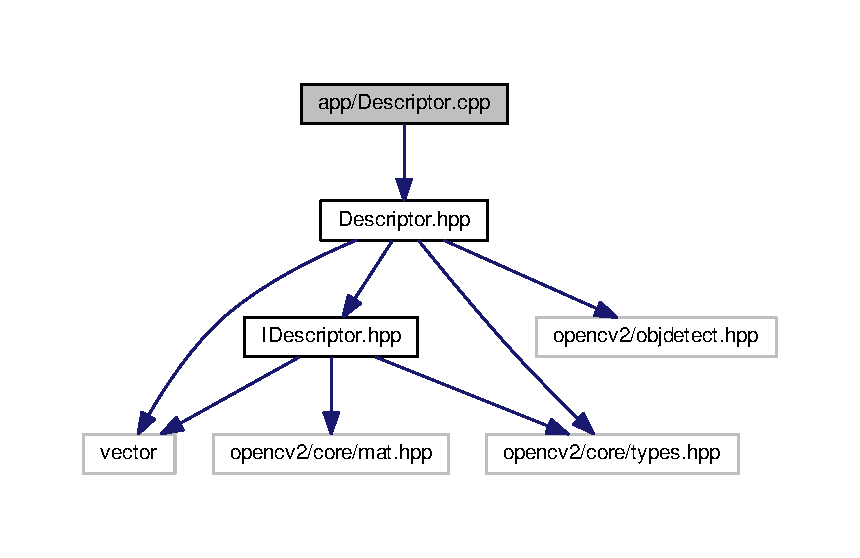
\includegraphics[width=350pt]{Descriptor_8cpp__incl}
\end{center}
\end{figure}

\hypertarget{HumanDetector_8cpp}{}\section{app/\+Human\+Detector.cpp File Reference}
\label{HumanDetector_8cpp}\index{app/\+Human\+Detector.\+cpp@{app/\+Human\+Detector.\+cpp}}
{\ttfamily \#include $<$Human\+Detector.\+hpp$>$}\\*
Include dependency graph for Human\+Detector.\+cpp\+:
\nopagebreak
\begin{figure}[H]
\begin{center}
\leavevmode
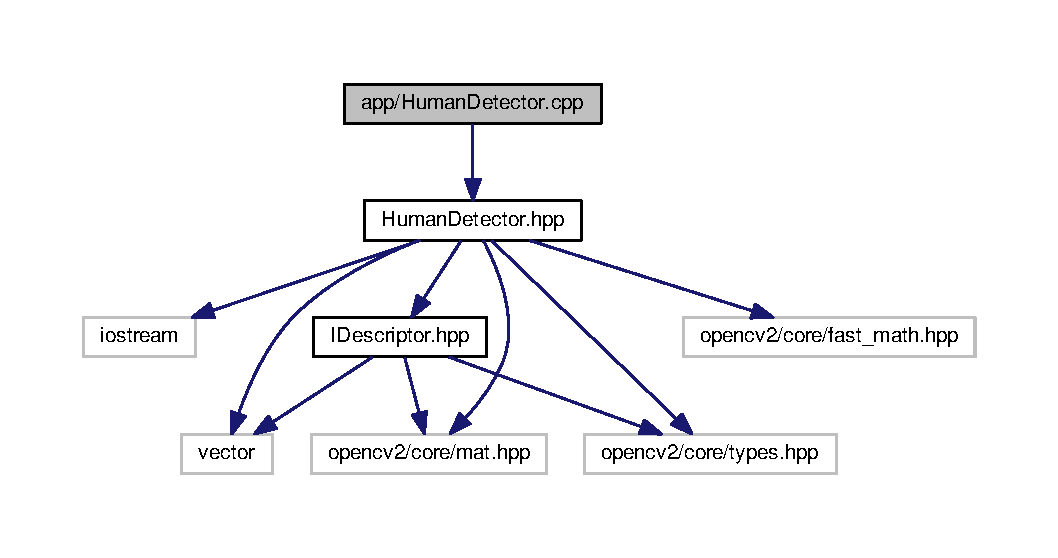
\includegraphics[width=350pt]{HumanDetector_8cpp__incl}
\end{center}
\end{figure}

\hypertarget{ImageInput_8cpp}{}\section{app/\+Image\+Input.cpp File Reference}
\label{ImageInput_8cpp}\index{app/\+Image\+Input.\+cpp@{app/\+Image\+Input.\+cpp}}
{\ttfamily \#include $<$Image\+Input.\+hpp$>$}\\*
Include dependency graph for Image\+Input.\+cpp\+:
\nopagebreak
\begin{figure}[H]
\begin{center}
\leavevmode
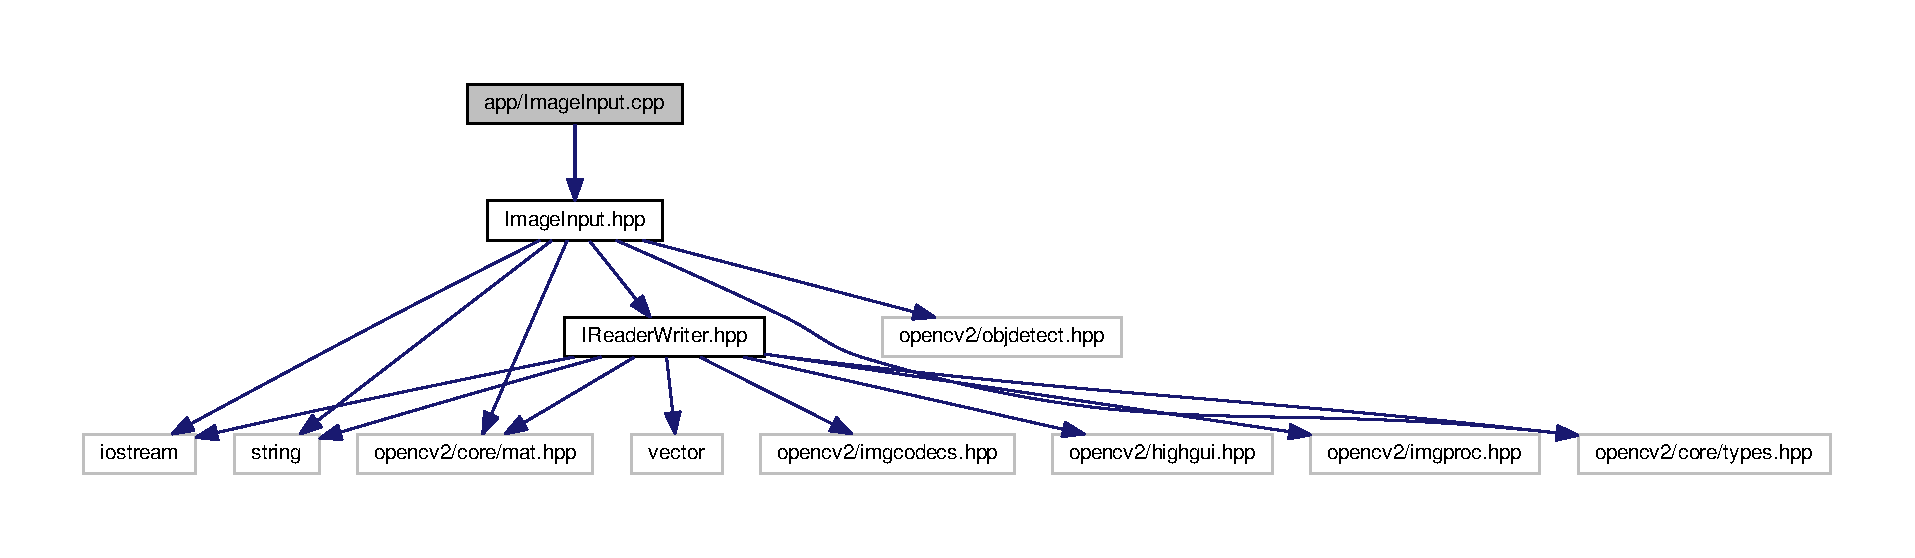
\includegraphics[width=350pt]{ImageInput_8cpp__incl}
\end{center}
\end{figure}

\hypertarget{ImageOutput_8cpp}{}\section{app/\+Image\+Output.cpp File Reference}
\label{ImageOutput_8cpp}\index{app/\+Image\+Output.\+cpp@{app/\+Image\+Output.\+cpp}}
{\ttfamily \#include $<$Image\+Output.\+hpp$>$}\\*
Include dependency graph for Image\+Output.\+cpp\+:
\nopagebreak
\begin{figure}[H]
\begin{center}
\leavevmode
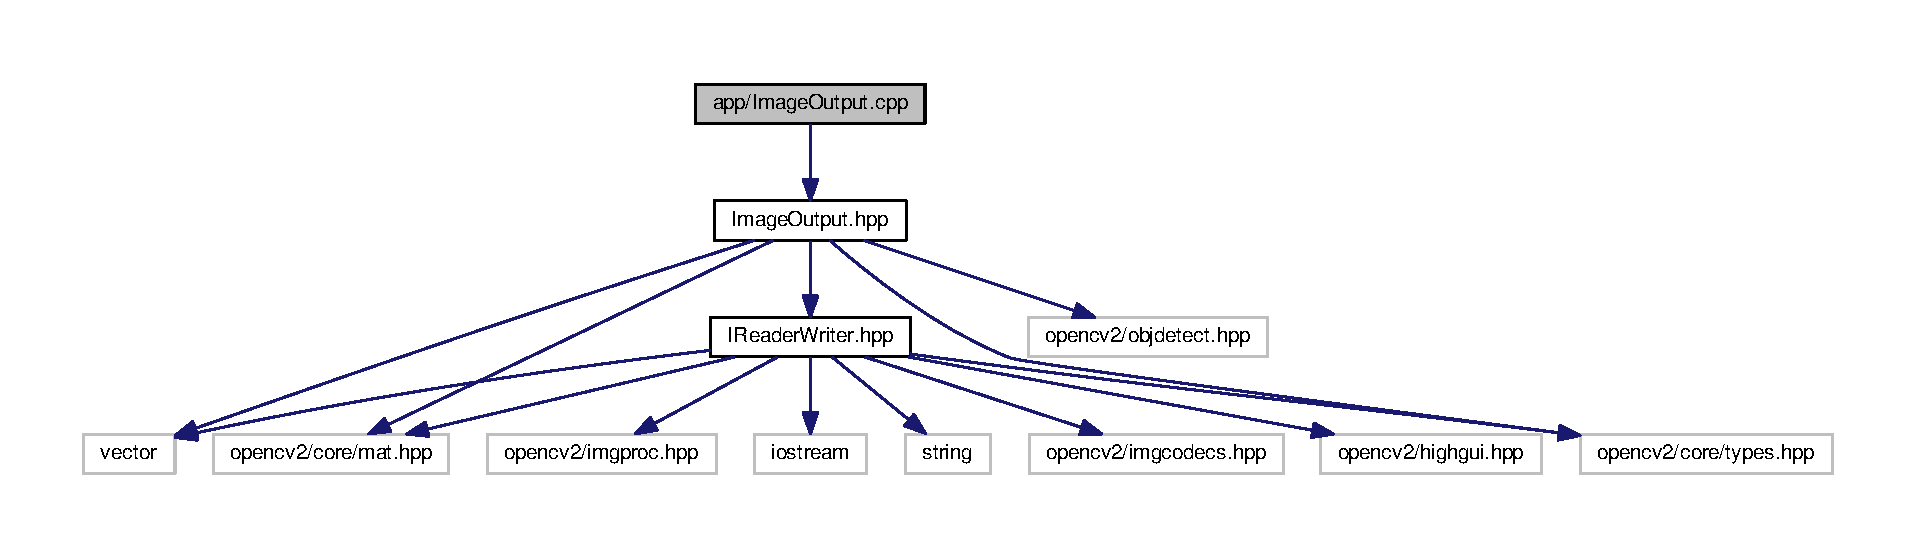
\includegraphics[width=350pt]{ImageOutput_8cpp__incl}
\end{center}
\end{figure}

\hypertarget{main_8cpp}{}\section{app/main.cpp File Reference}
\label{main_8cpp}\index{app/main.\+cpp@{app/main.\+cpp}}
{\ttfamily \#include $<$iostream$>$}\\*
{\ttfamily \#include $<$string$>$}\\*
{\ttfamily \#include $<$Human\+Detector.\+hpp$>$}\\*
{\ttfamily \#include $<$I\+Descriptor.\+hpp$>$}\\*
{\ttfamily \#include $<$Descriptor.\+hpp$>$}\\*
{\ttfamily \#include $<$Image\+Input.\+hpp$>$}\\*
{\ttfamily \#include $<$Image\+Output.\+hpp$>$}\\*
{\ttfamily \#include $<$Reader\+Writer.\+hpp$>$}\\*
{\ttfamily \#include $<$I\+Reader\+Writer.\+hpp$>$}\\*
{\ttfamily \#include $<$opencv2/imgcodecs.\+hpp$>$}\\*
{\ttfamily \#include $<$opencv2/core/mat.\+hpp$>$}\\*
{\ttfamily \#include $<$opencv2/core/types.\+hpp$>$}\\*
{\ttfamily \#include $<$opencv2/highgui.\+hpp$>$}\\*
Include dependency graph for main.\+cpp\+:
\nopagebreak
\begin{figure}[H]
\begin{center}
\leavevmode
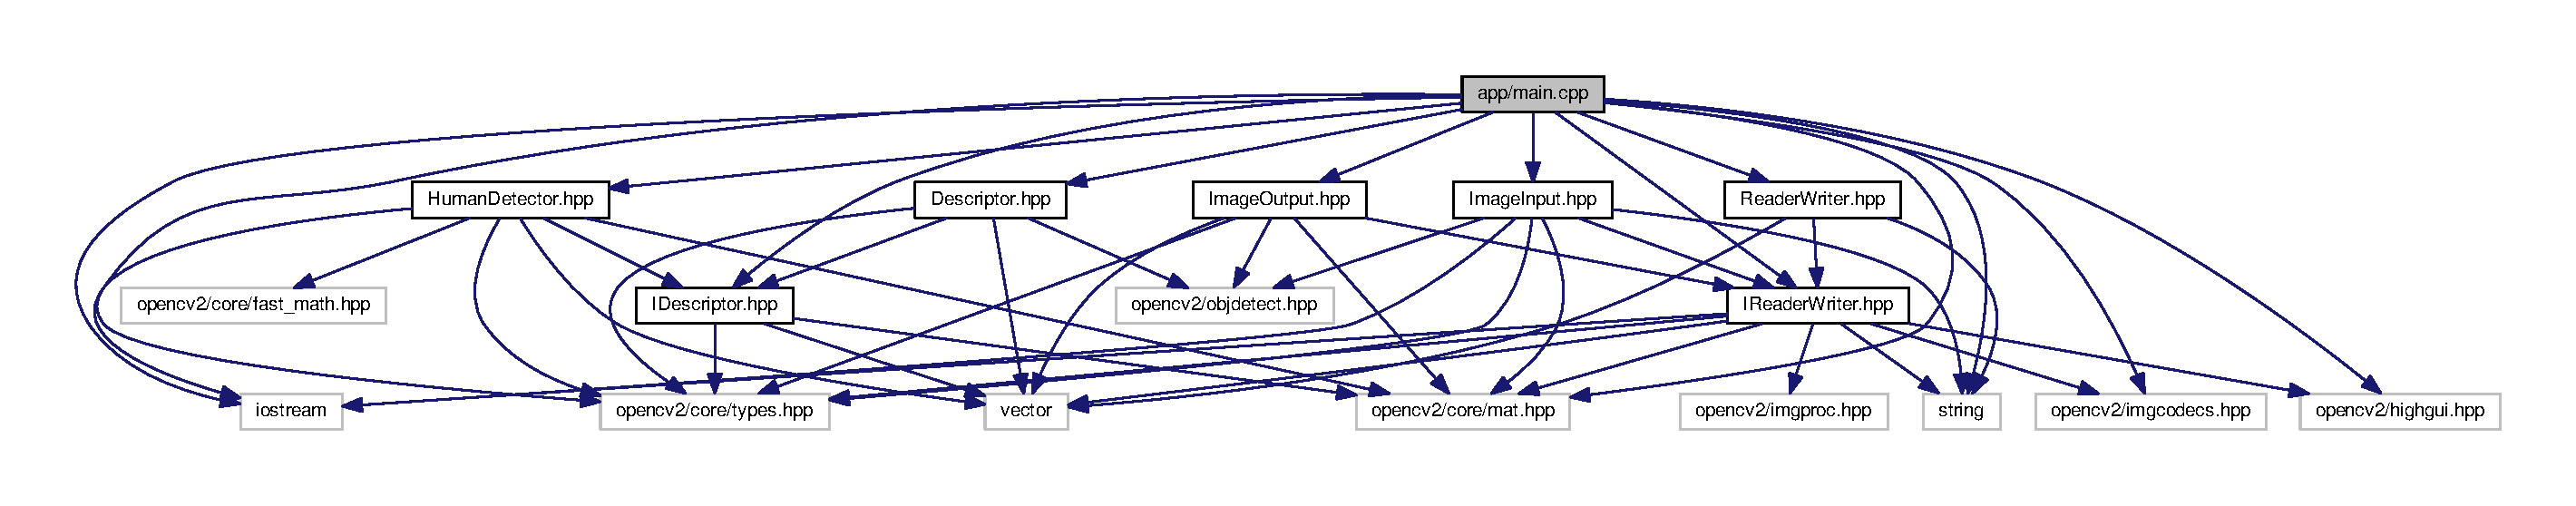
\includegraphics[width=350pt]{main_8cpp__incl}
\end{center}
\end{figure}
\subsection*{Functions}
\begin{DoxyCompactItemize}
\item 
int \hyperlink{main_8cpp_a3c04138a5bfe5d72780bb7e82a18e627}{main} (int argc, char $\ast$$\ast$argv)
\end{DoxyCompactItemize}


\subsection{Function Documentation}
\index{main.\+cpp@{main.\+cpp}!main@{main}}
\index{main@{main}!main.\+cpp@{main.\+cpp}}
\subsubsection[{\texorpdfstring{main(int argc, char $\ast$$\ast$argv)}{main(int argc, char **argv)}}]{\setlength{\rightskip}{0pt plus 5cm}int main (
\begin{DoxyParamCaption}
\item[{int}]{argc, }
\item[{char $\ast$$\ast$}]{argv}
\end{DoxyParamCaption}
)}\hypertarget{main_8cpp_a3c04138a5bfe5d72780bb7e82a18e627}{}\label{main_8cpp_a3c04138a5bfe5d72780bb7e82a18e627}

\hypertarget{ReaderWriter_8cpp}{}\section{app/\+Reader\+Writer.cpp File Reference}
\label{ReaderWriter_8cpp}\index{app/\+Reader\+Writer.\+cpp@{app/\+Reader\+Writer.\+cpp}}
{\ttfamily \#include $<$Reader\+Writer.\+hpp$>$}\\*
Include dependency graph for Reader\+Writer.\+cpp\+:
\nopagebreak
\begin{figure}[H]
\begin{center}
\leavevmode
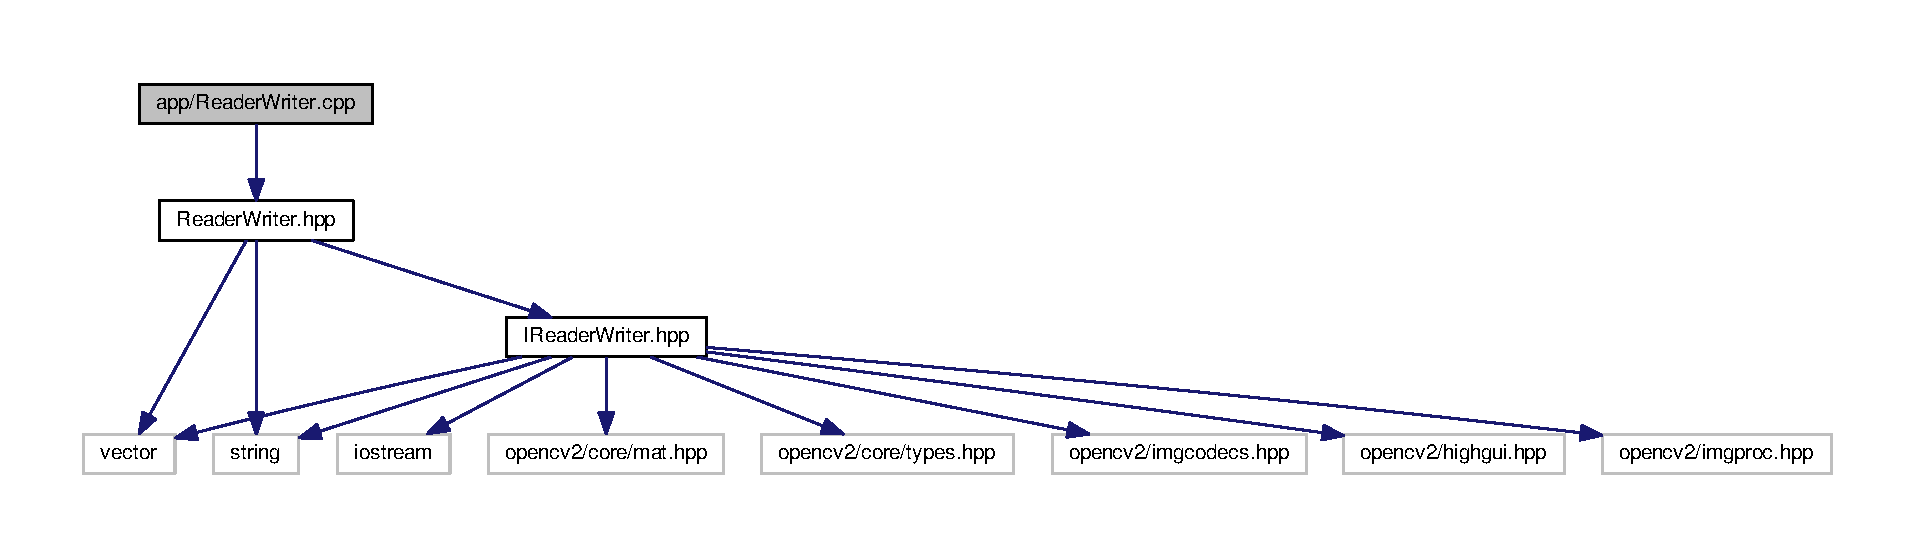
\includegraphics[width=350pt]{ReaderWriter_8cpp__incl}
\end{center}
\end{figure}

\hypertarget{Descriptor_8hpp}{}\section{include/\+Descriptor.hpp File Reference}
\label{Descriptor_8hpp}\index{include/\+Descriptor.\+hpp@{include/\+Descriptor.\+hpp}}
{\ttfamily \#include $<$vector$>$}\\*
{\ttfamily \#include $<$I\+Descriptor.\+hpp$>$}\\*
{\ttfamily \#include $<$opencv2/objdetect.\+hpp$>$}\\*
{\ttfamily \#include $<$opencv2/core/types.\+hpp$>$}\\*
Include dependency graph for Descriptor.\+hpp\+:
\nopagebreak
\begin{figure}[H]
\begin{center}
\leavevmode
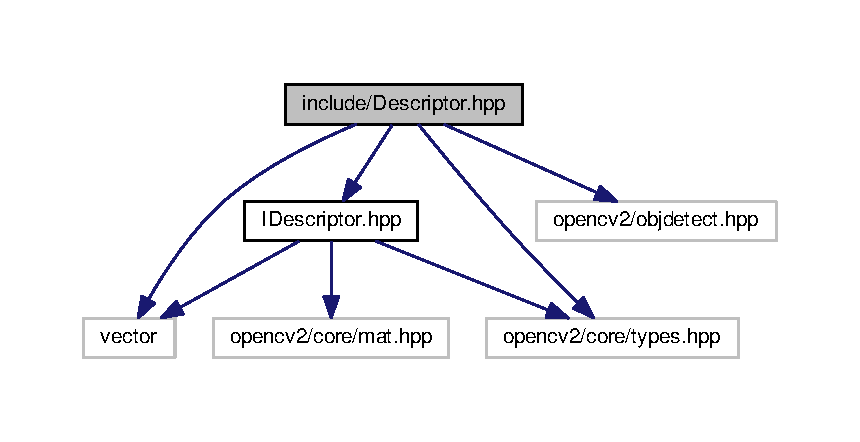
\includegraphics[width=350pt]{Descriptor_8hpp__incl}
\end{center}
\end{figure}
This graph shows which files directly or indirectly include this file\+:
\nopagebreak
\begin{figure}[H]
\begin{center}
\leavevmode
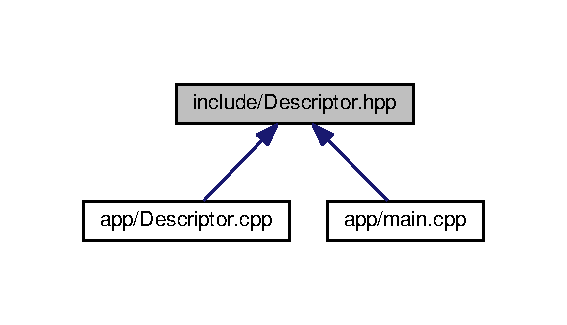
\includegraphics[width=272pt]{Descriptor_8hpp__dep__incl}
\end{center}
\end{figure}
\subsection*{Classes}
\begin{DoxyCompactItemize}
\item 
class \hyperlink{classDescriptor}{Descriptor}
\end{DoxyCompactItemize}

\hypertarget{HumanDetector_8hpp}{}\section{include/\+Human\+Detector.hpp File Reference}
\label{HumanDetector_8hpp}\index{include/\+Human\+Detector.\+hpp@{include/\+Human\+Detector.\+hpp}}
{\ttfamily \#include $<$iostream$>$}\\*
{\ttfamily \#include $<$vector$>$}\\*
{\ttfamily \#include $<$I\+Descriptor.\+hpp$>$}\\*
{\ttfamily \#include $<$opencv2/core/mat.\+hpp$>$}\\*
{\ttfamily \#include $<$opencv2/core/types.\+hpp$>$}\\*
{\ttfamily \#include $<$opencv2/core/fast\+\_\+math.\+hpp$>$}\\*
Include dependency graph for Human\+Detector.\+hpp\+:
\nopagebreak
\begin{figure}[H]
\begin{center}
\leavevmode
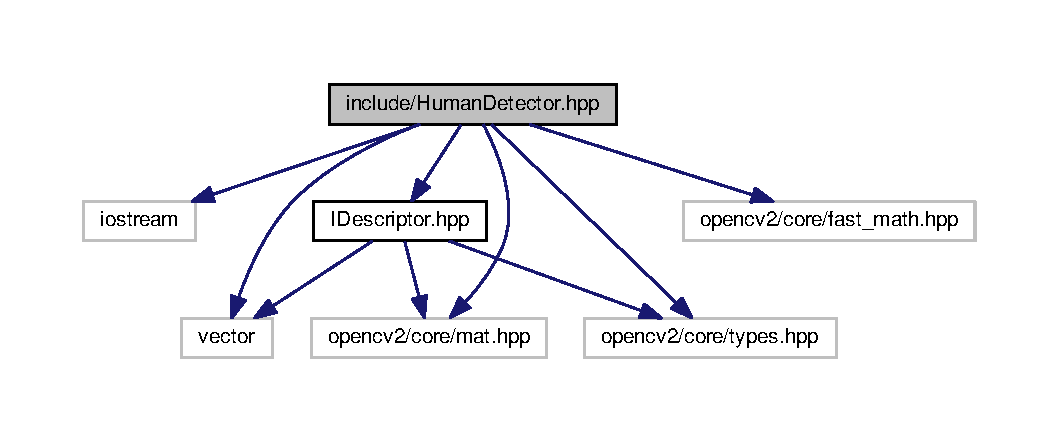
\includegraphics[width=350pt]{HumanDetector_8hpp__incl}
\end{center}
\end{figure}
This graph shows which files directly or indirectly include this file\+:
\nopagebreak
\begin{figure}[H]
\begin{center}
\leavevmode
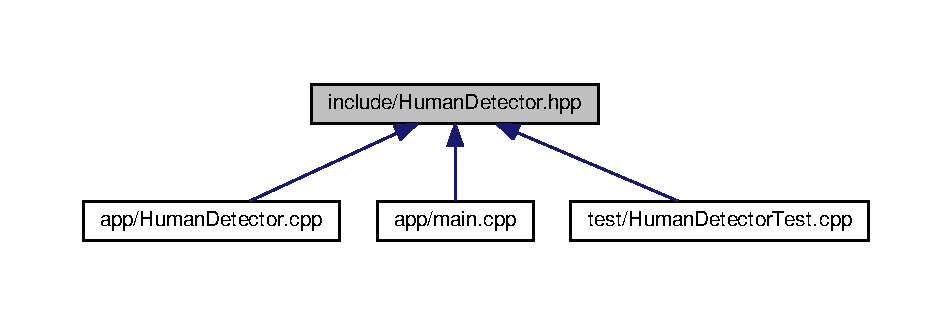
\includegraphics[width=350pt]{HumanDetector_8hpp__dep__incl}
\end{center}
\end{figure}
\subsection*{Classes}
\begin{DoxyCompactItemize}
\item 
class \hyperlink{classHumanDetector}{Human\+Detector}
\end{DoxyCompactItemize}

\hypertarget{IDescriptor_8hpp}{}\section{include/\+I\+Descriptor.hpp File Reference}
\label{IDescriptor_8hpp}\index{include/\+I\+Descriptor.\+hpp@{include/\+I\+Descriptor.\+hpp}}
{\ttfamily \#include $<$vector$>$}\\*
{\ttfamily \#include $<$opencv2/core/mat.\+hpp$>$}\\*
{\ttfamily \#include $<$opencv2/core/types.\+hpp$>$}\\*
Include dependency graph for I\+Descriptor.\+hpp\+:
\nopagebreak
\begin{figure}[H]
\begin{center}
\leavevmode
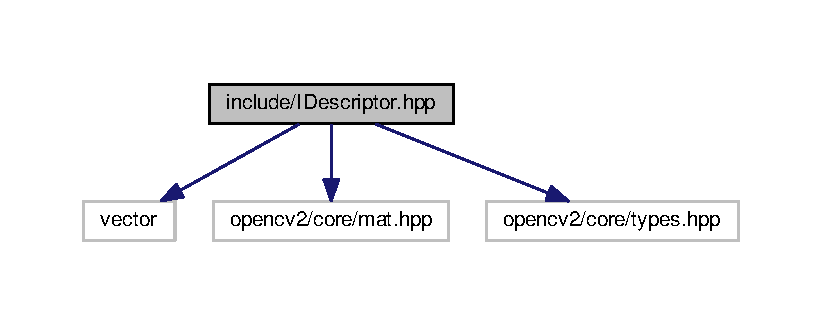
\includegraphics[width=350pt]{IDescriptor_8hpp__incl}
\end{center}
\end{figure}
This graph shows which files directly or indirectly include this file\+:
\nopagebreak
\begin{figure}[H]
\begin{center}
\leavevmode
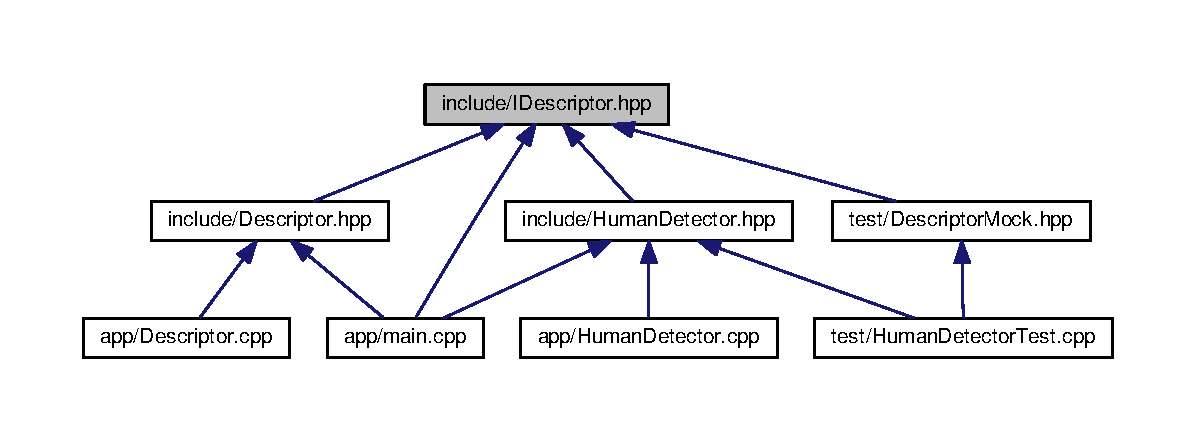
\includegraphics[width=350pt]{IDescriptor_8hpp__dep__incl}
\end{center}
\end{figure}
\subsection*{Classes}
\begin{DoxyCompactItemize}
\item 
class \hyperlink{classIDescriptor}{I\+Descriptor}
\end{DoxyCompactItemize}

\hypertarget{ImageInput_8hpp}{}\section{include/\+Image\+Input.hpp File Reference}
\label{ImageInput_8hpp}\index{include/\+Image\+Input.\+hpp@{include/\+Image\+Input.\+hpp}}
{\ttfamily \#include $<$iostream$>$}\\*
{\ttfamily \#include $<$string$>$}\\*
{\ttfamily \#include $<$I\+Reader\+Writer.\+hpp$>$}\\*
{\ttfamily \#include $<$opencv2/objdetect.\+hpp$>$}\\*
{\ttfamily \#include $<$opencv2/core/mat.\+hpp$>$}\\*
{\ttfamily \#include $<$opencv2/core/types.\+hpp$>$}\\*
Include dependency graph for Image\+Input.\+hpp\+:
\nopagebreak
\begin{figure}[H]
\begin{center}
\leavevmode
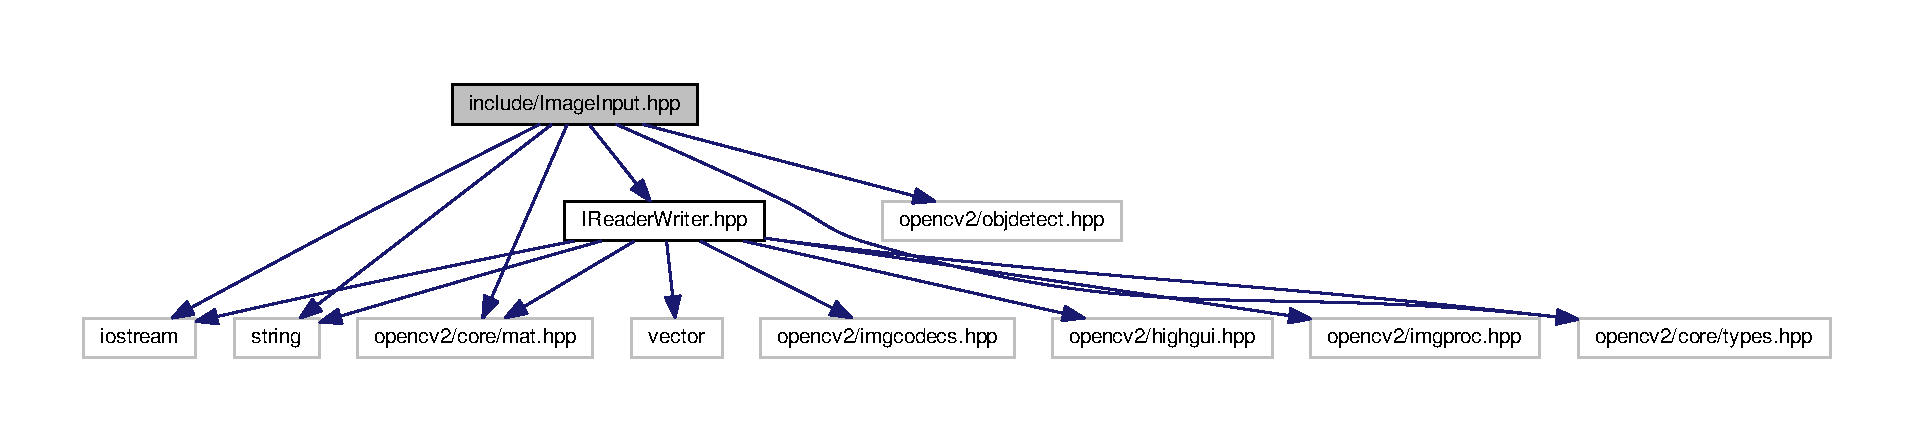
\includegraphics[width=350pt]{ImageInput_8hpp__incl}
\end{center}
\end{figure}
This graph shows which files directly or indirectly include this file\+:
\nopagebreak
\begin{figure}[H]
\begin{center}
\leavevmode
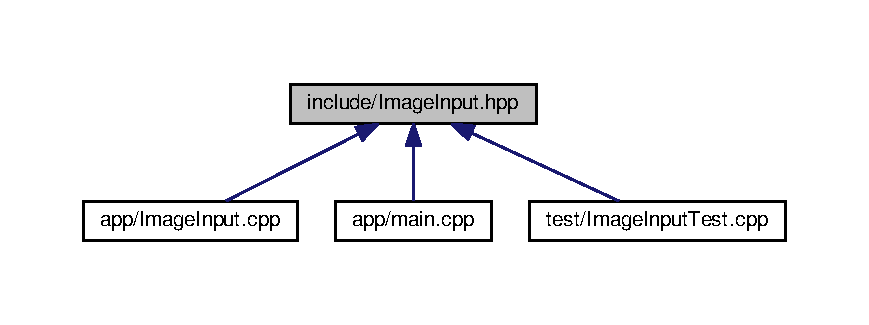
\includegraphics[width=350pt]{ImageInput_8hpp__dep__incl}
\end{center}
\end{figure}
\subsection*{Classes}
\begin{DoxyCompactItemize}
\item 
class \hyperlink{classImageInput}{Image\+Input}
\end{DoxyCompactItemize}

\hypertarget{ImageOutput_8hpp}{}\section{include/\+Image\+Output.hpp File Reference}
\label{ImageOutput_8hpp}\index{include/\+Image\+Output.\+hpp@{include/\+Image\+Output.\+hpp}}
{\ttfamily \#include $<$vector$>$}\\*
{\ttfamily \#include $<$I\+Reader\+Writer.\+hpp$>$}\\*
{\ttfamily \#include $<$opencv2/objdetect.\+hpp$>$}\\*
{\ttfamily \#include $<$opencv2/core/mat.\+hpp$>$}\\*
{\ttfamily \#include $<$opencv2/core/types.\+hpp$>$}\\*
Include dependency graph for Image\+Output.\+hpp\+:
\nopagebreak
\begin{figure}[H]
\begin{center}
\leavevmode
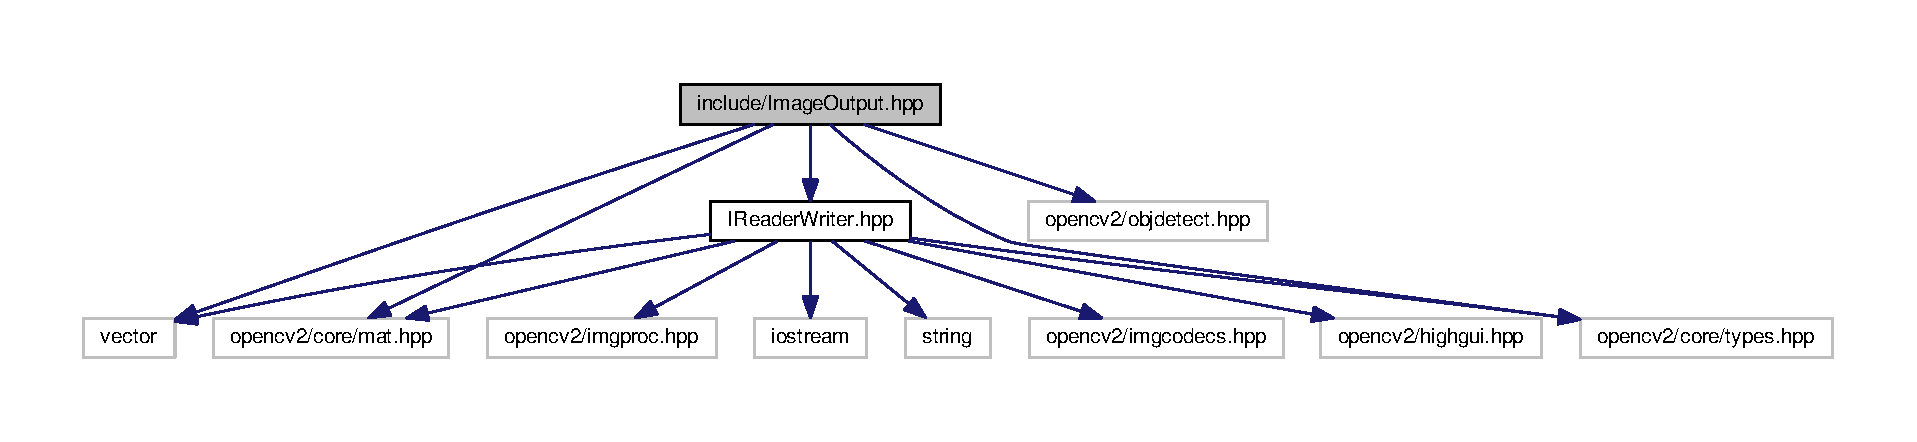
\includegraphics[width=350pt]{ImageOutput_8hpp__incl}
\end{center}
\end{figure}
This graph shows which files directly or indirectly include this file\+:
\nopagebreak
\begin{figure}[H]
\begin{center}
\leavevmode
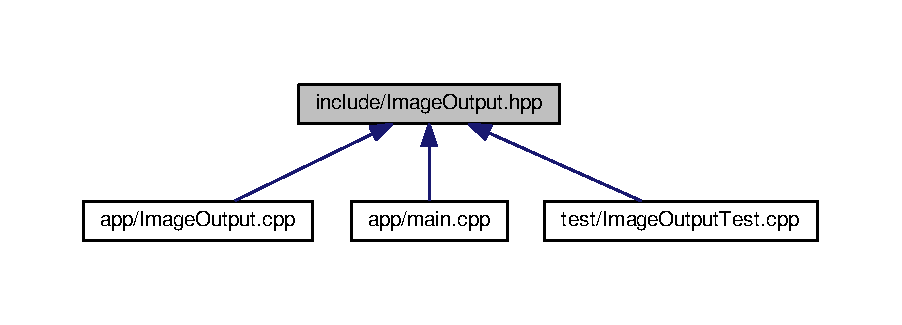
\includegraphics[width=350pt]{ImageOutput_8hpp__dep__incl}
\end{center}
\end{figure}
\subsection*{Classes}
\begin{DoxyCompactItemize}
\item 
class \hyperlink{classImageOutput}{Image\+Output}
\end{DoxyCompactItemize}

\hypertarget{IReaderWriter_8hpp}{}\section{include/\+I\+Reader\+Writer.hpp File Reference}
\label{IReaderWriter_8hpp}\index{include/\+I\+Reader\+Writer.\+hpp@{include/\+I\+Reader\+Writer.\+hpp}}
{\ttfamily \#include $<$vector$>$}\\*
{\ttfamily \#include $<$iostream$>$}\\*
{\ttfamily \#include $<$string$>$}\\*
{\ttfamily \#include $<$opencv2/core/mat.\+hpp$>$}\\*
{\ttfamily \#include $<$opencv2/core/types.\+hpp$>$}\\*
{\ttfamily \#include $<$opencv2/imgcodecs.\+hpp$>$}\\*
{\ttfamily \#include $<$opencv2/highgui.\+hpp$>$}\\*
{\ttfamily \#include $<$opencv2/imgproc.\+hpp$>$}\\*
Include dependency graph for I\+Reader\+Writer.\+hpp\+:
\nopagebreak
\begin{figure}[H]
\begin{center}
\leavevmode
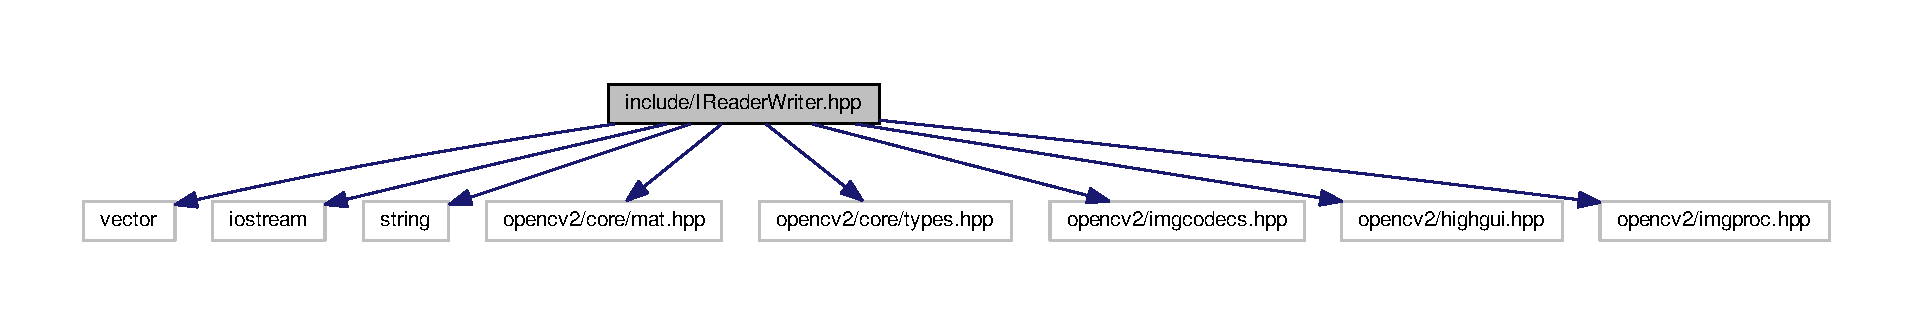
\includegraphics[width=350pt]{IReaderWriter_8hpp__incl}
\end{center}
\end{figure}
This graph shows which files directly or indirectly include this file\+:
\nopagebreak
\begin{figure}[H]
\begin{center}
\leavevmode
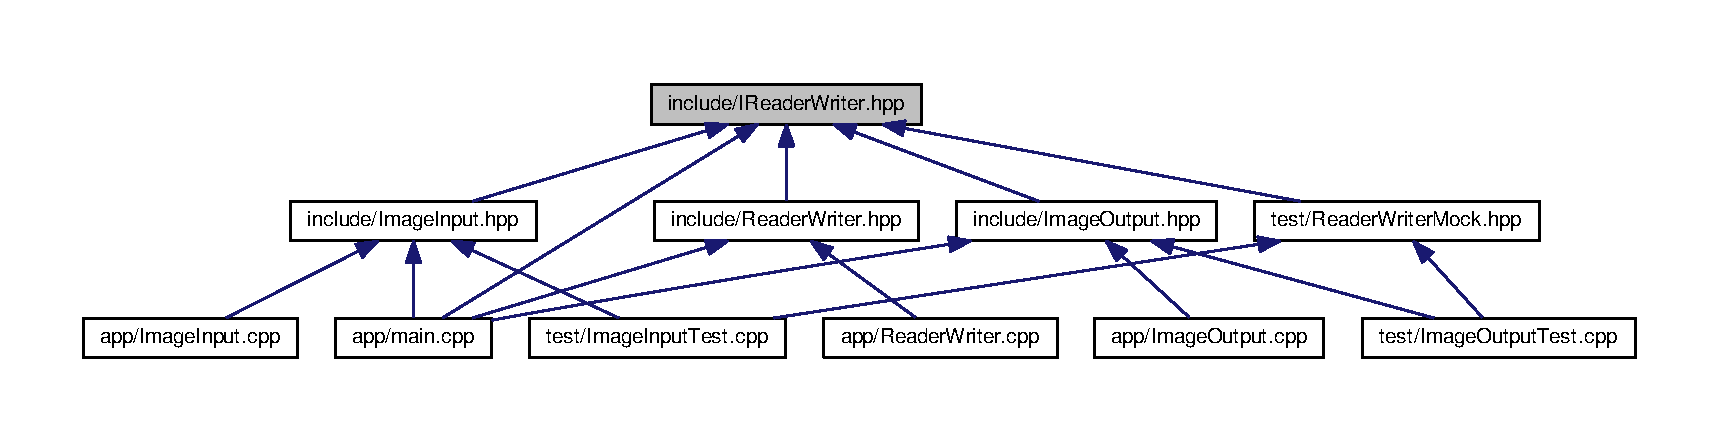
\includegraphics[width=350pt]{IReaderWriter_8hpp__dep__incl}
\end{center}
\end{figure}
\subsection*{Classes}
\begin{DoxyCompactItemize}
\item 
class \hyperlink{classIReaderWriter}{I\+Reader\+Writer}
\end{DoxyCompactItemize}

\hypertarget{ReaderWriter_8hpp}{}\section{include/\+Reader\+Writer.hpp File Reference}
\label{ReaderWriter_8hpp}\index{include/\+Reader\+Writer.\+hpp@{include/\+Reader\+Writer.\+hpp}}
{\ttfamily \#include $<$vector$>$}\\*
{\ttfamily \#include $<$string$>$}\\*
{\ttfamily \#include $<$I\+Reader\+Writer.\+hpp$>$}\\*
Include dependency graph for Reader\+Writer.\+hpp\+:
\nopagebreak
\begin{figure}[H]
\begin{center}
\leavevmode
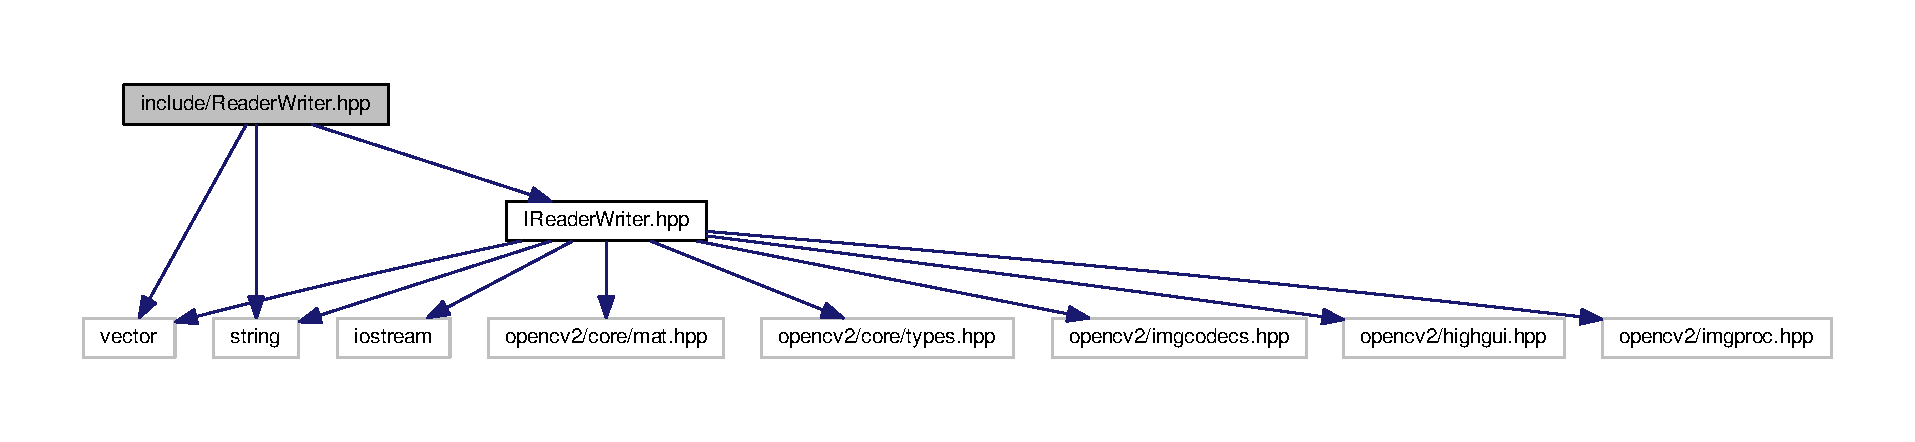
\includegraphics[width=350pt]{ReaderWriter_8hpp__incl}
\end{center}
\end{figure}
This graph shows which files directly or indirectly include this file\+:
\nopagebreak
\begin{figure}[H]
\begin{center}
\leavevmode
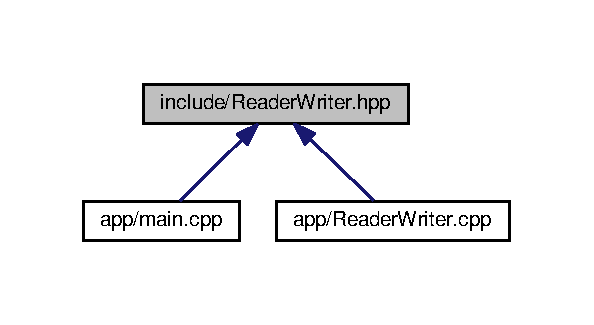
\includegraphics[width=285pt]{ReaderWriter_8hpp__dep__incl}
\end{center}
\end{figure}
\subsection*{Classes}
\begin{DoxyCompactItemize}
\item 
class \hyperlink{classReaderWriter}{Reader\+Writer}
\end{DoxyCompactItemize}

\hypertarget{readme_8md}{}\section{readme.\+md File Reference}
\label{readme_8md}\index{readme.\+md@{readme.\+md}}

\hypertarget{CPPCheckResult_8txt}{}\section{reports/\+C\+P\+P\+Check\+Result.txt File Reference}
\label{CPPCheckResult_8txt}\index{reports/\+C\+P\+P\+Check\+Result.\+txt@{reports/\+C\+P\+P\+Check\+Result.\+txt}}

\hypertarget{CppLintResult_8txt}{}\section{reports/\+Cpp\+Lint\+Result.txt File Reference}
\label{CppLintResult_8txt}\index{reports/\+Cpp\+Lint\+Result.\+txt@{reports/\+Cpp\+Lint\+Result.\+txt}}

\hypertarget{DescriptorMock_8hpp}{}\section{test/\+Descriptor\+Mock.hpp File Reference}
\label{DescriptorMock_8hpp}\index{test/\+Descriptor\+Mock.\+hpp@{test/\+Descriptor\+Mock.\+hpp}}
{\ttfamily \#include $<$vector$>$}\\*
{\ttfamily \#include $<$I\+Descriptor.\+hpp$>$}\\*
{\ttfamily \#include $<$opencv2/core/mat.\+hpp$>$}\\*
{\ttfamily \#include $<$opencv2/core/types.\+hpp$>$}\\*
Include dependency graph for Descriptor\+Mock.\+hpp\+:
\nopagebreak
\begin{figure}[H]
\begin{center}
\leavevmode
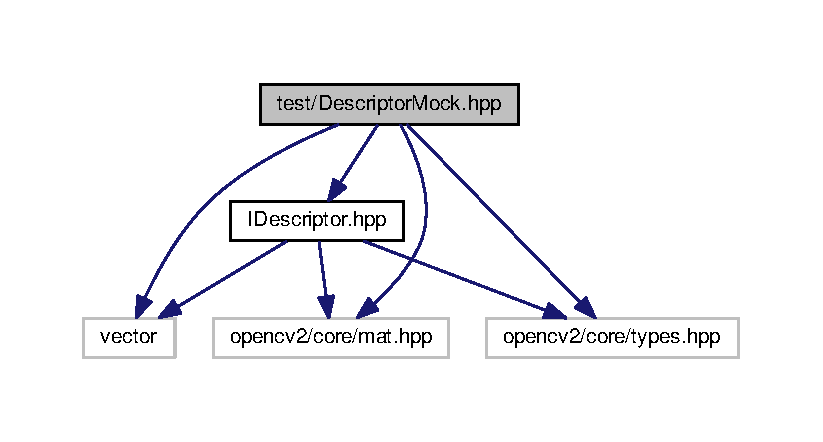
\includegraphics[width=350pt]{DescriptorMock_8hpp__incl}
\end{center}
\end{figure}
This graph shows which files directly or indirectly include this file\+:
\nopagebreak
\begin{figure}[H]
\begin{center}
\leavevmode
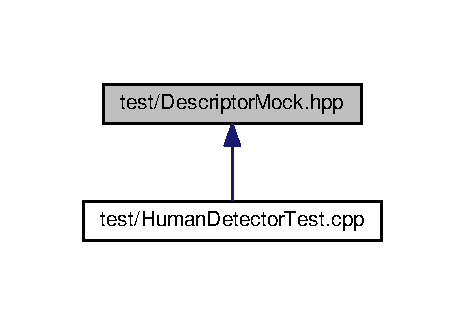
\includegraphics[width=223pt]{DescriptorMock_8hpp__dep__incl}
\end{center}
\end{figure}
\subsection*{Classes}
\begin{DoxyCompactItemize}
\item 
class \hyperlink{classDescriptorMock}{Descriptor\+Mock}
\end{DoxyCompactItemize}

\hypertarget{HumanDetectorTest_8cpp}{}\section{test/\+Human\+Detector\+Test.cpp File Reference}
\label{HumanDetectorTest_8cpp}\index{test/\+Human\+Detector\+Test.\+cpp@{test/\+Human\+Detector\+Test.\+cpp}}
{\ttfamily \#include $<$gtest/gtest.\+h$>$}\\*
{\ttfamily \#include $<$Human\+Detector.\+hpp$>$}\\*
{\ttfamily \#include $<$Descriptor\+Mock.\+hpp$>$}\\*
{\ttfamily \#include $<$opencv2/imgcodecs.\+hpp$>$}\\*
{\ttfamily \#include $<$opencv2/core/mat.\+hpp$>$}\\*
{\ttfamily \#include $<$opencv2/core/types.\+hpp$>$}\\*
Include dependency graph for Human\+Detector\+Test.\+cpp\+:
\nopagebreak
\begin{figure}[H]
\begin{center}
\leavevmode
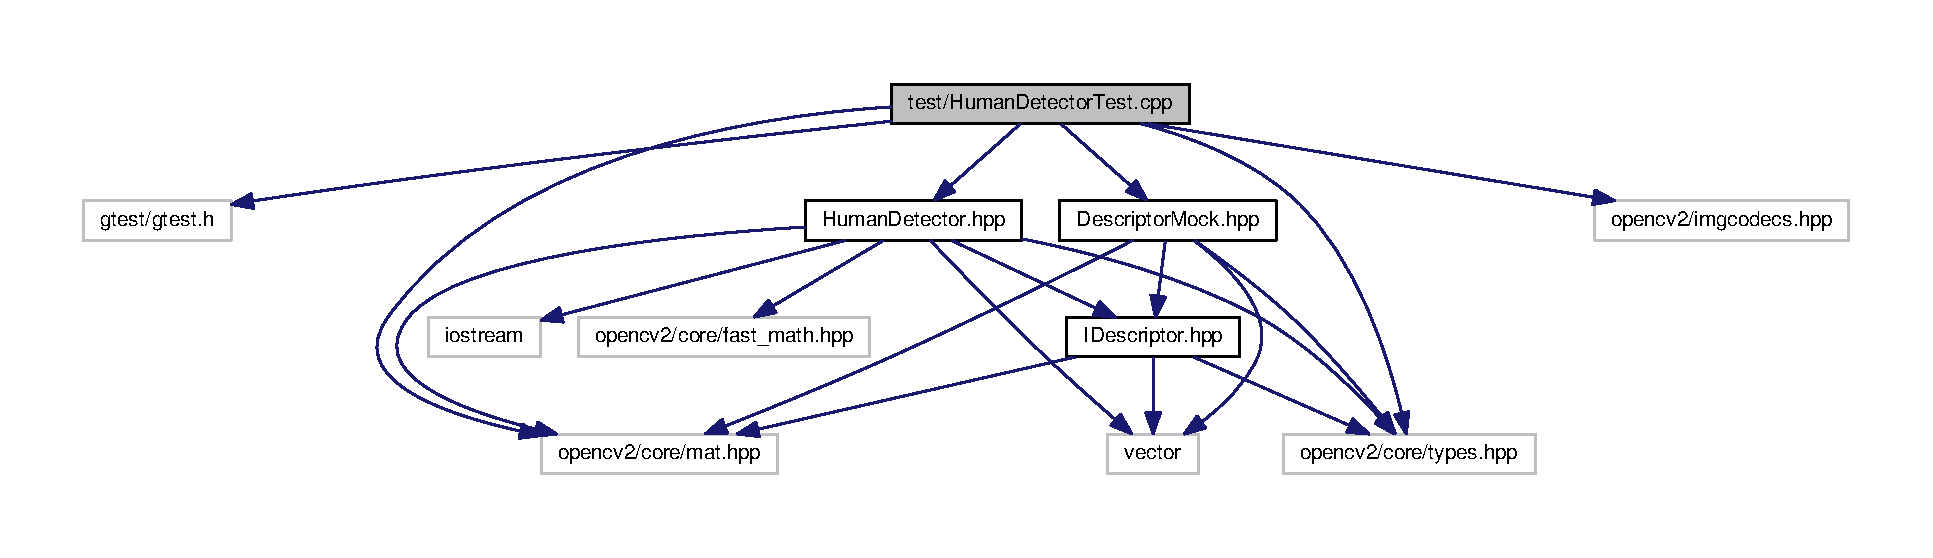
\includegraphics[width=350pt]{HumanDetectorTest_8cpp__incl}
\end{center}
\end{figure}
\subsection*{Functions}
\begin{DoxyCompactItemize}
\item 
\hyperlink{HumanDetectorTest_8cpp_a870aec98a750c62d2050b539b2e128db}{T\+E\+ST} (human\+Detector, one\+\_\+human\+\_\+found)
\item 
\hyperlink{HumanDetectorTest_8cpp_ac0a24d8b7012c28e973d96ba71a989bb}{T\+E\+ST} (human\+Detector, should\+\_\+reduce\+\_\+boundary)
\end{DoxyCompactItemize}


\subsection{Function Documentation}
\index{Human\+Detector\+Test.\+cpp@{Human\+Detector\+Test.\+cpp}!T\+E\+ST@{T\+E\+ST}}
\index{T\+E\+ST@{T\+E\+ST}!Human\+Detector\+Test.\+cpp@{Human\+Detector\+Test.\+cpp}}
\subsubsection[{\texorpdfstring{T\+E\+S\+T(human\+Detector, one\+\_\+human\+\_\+found)}{TEST(humanDetector, one_human_found)}}]{\setlength{\rightskip}{0pt plus 5cm}T\+E\+ST (
\begin{DoxyParamCaption}
\item[{human\+Detector}]{, }
\item[{one\+\_\+human\+\_\+found}]{}
\end{DoxyParamCaption}
)}\hypertarget{HumanDetectorTest_8cpp_a870aec98a750c62d2050b539b2e128db}{}\label{HumanDetectorTest_8cpp_a870aec98a750c62d2050b539b2e128db}
\index{Human\+Detector\+Test.\+cpp@{Human\+Detector\+Test.\+cpp}!T\+E\+ST@{T\+E\+ST}}
\index{T\+E\+ST@{T\+E\+ST}!Human\+Detector\+Test.\+cpp@{Human\+Detector\+Test.\+cpp}}
\subsubsection[{\texorpdfstring{T\+E\+S\+T(human\+Detector, should\+\_\+reduce\+\_\+boundary)}{TEST(humanDetector, should_reduce_boundary)}}]{\setlength{\rightskip}{0pt plus 5cm}T\+E\+ST (
\begin{DoxyParamCaption}
\item[{human\+Detector}]{, }
\item[{should\+\_\+reduce\+\_\+boundary}]{}
\end{DoxyParamCaption}
)}\hypertarget{HumanDetectorTest_8cpp_ac0a24d8b7012c28e973d96ba71a989bb}{}\label{HumanDetectorTest_8cpp_ac0a24d8b7012c28e973d96ba71a989bb}

\hypertarget{ImageInputTest_8cpp}{}\section{test/\+Image\+Input\+Test.cpp File Reference}
\label{ImageInputTest_8cpp}\index{test/\+Image\+Input\+Test.\+cpp@{test/\+Image\+Input\+Test.\+cpp}}
{\ttfamily \#include $<$gtest/gtest.\+h$>$}\\*
{\ttfamily \#include $<$exception$>$}\\*
{\ttfamily \#include $<$Image\+Input.\+hpp$>$}\\*
{\ttfamily \#include $<$Reader\+Writer\+Mock.\+hpp$>$}\\*
Include dependency graph for Image\+Input\+Test.\+cpp\+:
\nopagebreak
\begin{figure}[H]
\begin{center}
\leavevmode
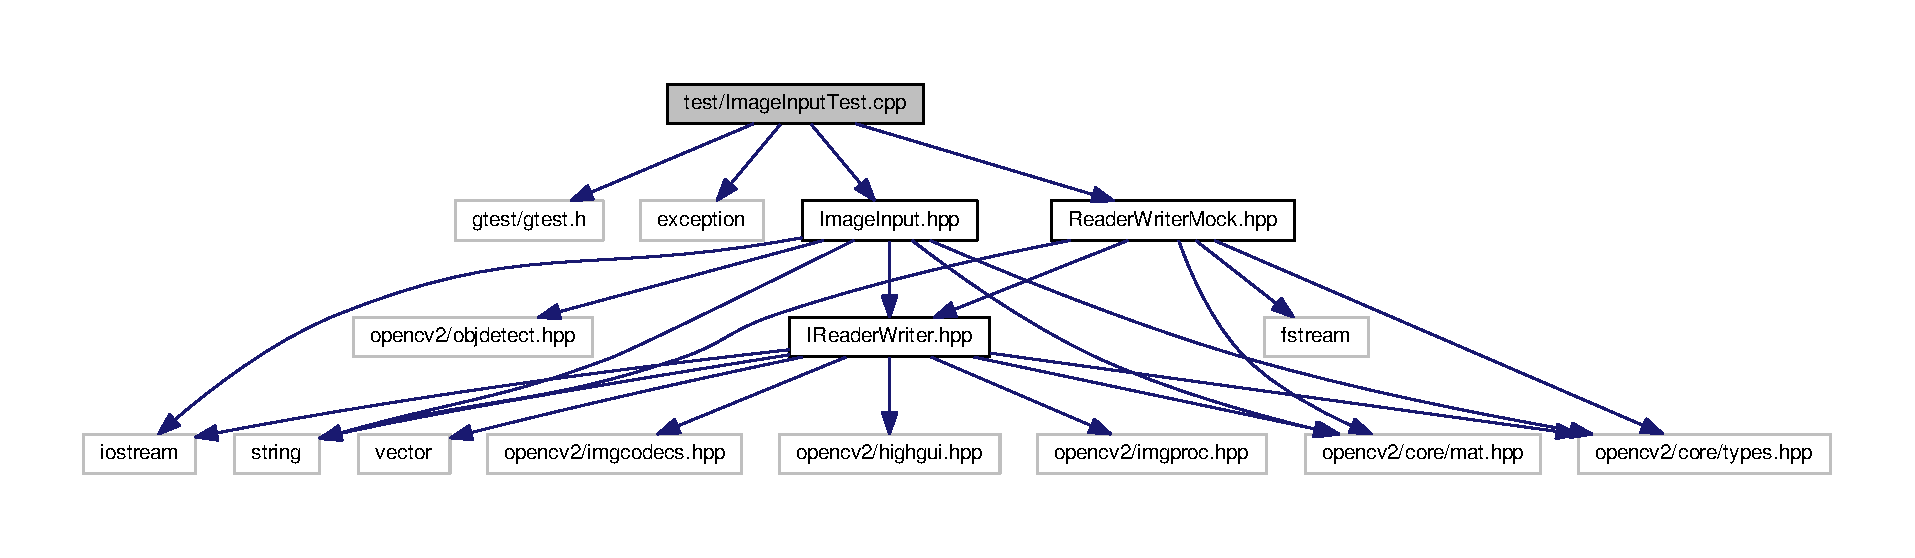
\includegraphics[width=350pt]{ImageInputTest_8cpp__incl}
\end{center}
\end{figure}
\subsection*{Functions}
\begin{DoxyCompactItemize}
\item 
\hyperlink{ImageInputTest_8cpp_a8567e25ad2abdcfd7cedfe1ce52be98c}{T\+E\+ST} (image\+Input, valid\+File)
\item 
\hyperlink{ImageInputTest_8cpp_a61cdcff79323e6f831d44cbad84e6f2f}{T\+E\+ST} (image\+Input, invalid\+File)
\end{DoxyCompactItemize}


\subsection{Function Documentation}
\index{Image\+Input\+Test.\+cpp@{Image\+Input\+Test.\+cpp}!T\+E\+ST@{T\+E\+ST}}
\index{T\+E\+ST@{T\+E\+ST}!Image\+Input\+Test.\+cpp@{Image\+Input\+Test.\+cpp}}
\subsubsection[{\texorpdfstring{T\+E\+S\+T(image\+Input, valid\+File)}{TEST(imageInput, validFile)}}]{\setlength{\rightskip}{0pt plus 5cm}T\+E\+ST (
\begin{DoxyParamCaption}
\item[{image\+Input}]{, }
\item[{valid\+File}]{}
\end{DoxyParamCaption}
)}\hypertarget{ImageInputTest_8cpp_a8567e25ad2abdcfd7cedfe1ce52be98c}{}\label{ImageInputTest_8cpp_a8567e25ad2abdcfd7cedfe1ce52be98c}
\index{Image\+Input\+Test.\+cpp@{Image\+Input\+Test.\+cpp}!T\+E\+ST@{T\+E\+ST}}
\index{T\+E\+ST@{T\+E\+ST}!Image\+Input\+Test.\+cpp@{Image\+Input\+Test.\+cpp}}
\subsubsection[{\texorpdfstring{T\+E\+S\+T(image\+Input, invalid\+File)}{TEST(imageInput, invalidFile)}}]{\setlength{\rightskip}{0pt plus 5cm}T\+E\+ST (
\begin{DoxyParamCaption}
\item[{image\+Input}]{, }
\item[{invalid\+File}]{}
\end{DoxyParamCaption}
)}\hypertarget{ImageInputTest_8cpp_a61cdcff79323e6f831d44cbad84e6f2f}{}\label{ImageInputTest_8cpp_a61cdcff79323e6f831d44cbad84e6f2f}

\hypertarget{ImageOutputTest_8cpp}{}\section{test/\+Image\+Output\+Test.cpp File Reference}
\label{ImageOutputTest_8cpp}\index{test/\+Image\+Output\+Test.\+cpp@{test/\+Image\+Output\+Test.\+cpp}}
{\ttfamily \#include $<$gtest/gtest.\+h$>$}\\*
{\ttfamily \#include $<$Image\+Output.\+hpp$>$}\\*
{\ttfamily \#include $<$Reader\+Writer\+Mock.\+hpp$>$}\\*
Include dependency graph for Image\+Output\+Test.\+cpp\+:
\nopagebreak
\begin{figure}[H]
\begin{center}
\leavevmode
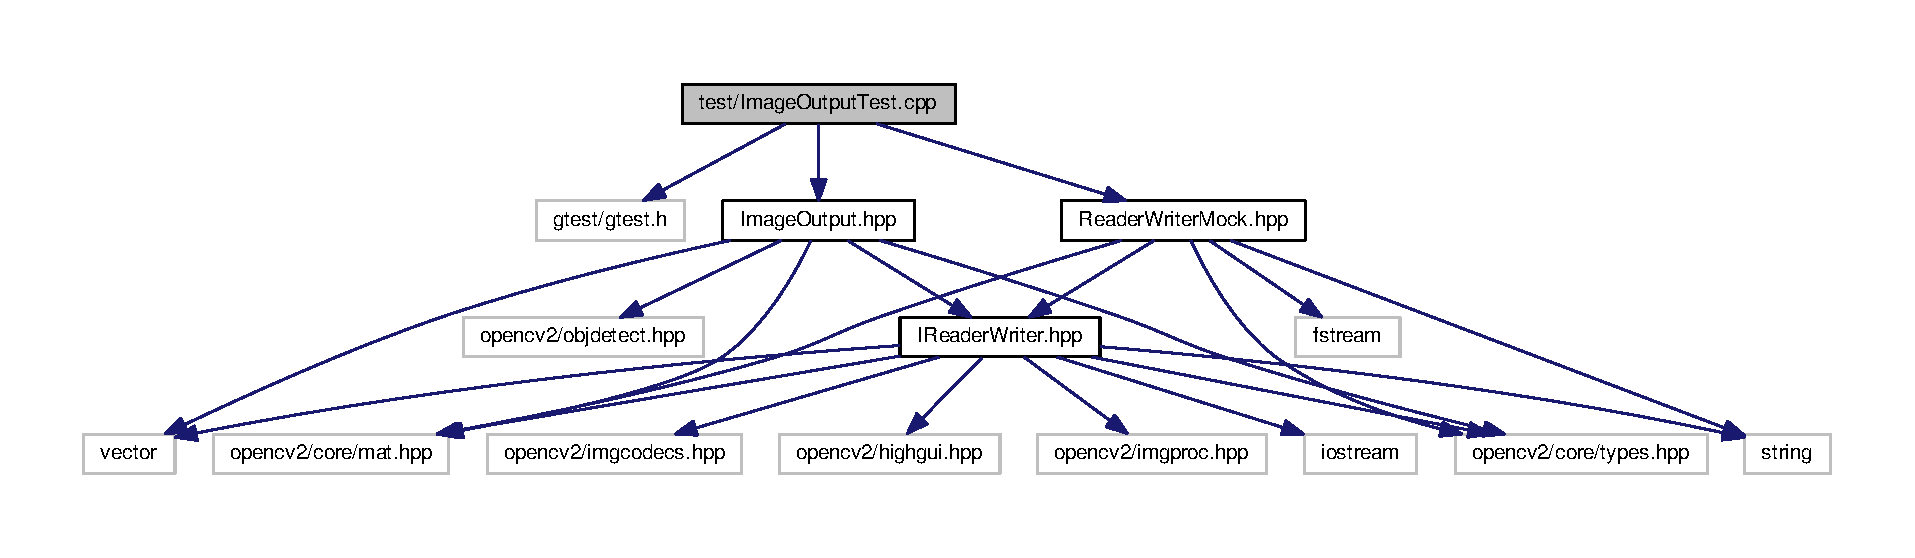
\includegraphics[width=350pt]{ImageOutputTest_8cpp__incl}
\end{center}
\end{figure}
\subsection*{Functions}
\begin{DoxyCompactItemize}
\item 
\hyperlink{ImageOutputTest_8cpp_a79114fafd07b03550d01bdc3187e22a9}{T\+E\+ST} (image\+Output, draw\+Boundary)
\end{DoxyCompactItemize}


\subsection{Function Documentation}
\index{Image\+Output\+Test.\+cpp@{Image\+Output\+Test.\+cpp}!T\+E\+ST@{T\+E\+ST}}
\index{T\+E\+ST@{T\+E\+ST}!Image\+Output\+Test.\+cpp@{Image\+Output\+Test.\+cpp}}
\subsubsection[{\texorpdfstring{T\+E\+S\+T(image\+Output, draw\+Boundary)}{TEST(imageOutput, drawBoundary)}}]{\setlength{\rightskip}{0pt plus 5cm}T\+E\+ST (
\begin{DoxyParamCaption}
\item[{image\+Output}]{, }
\item[{draw\+Boundary}]{}
\end{DoxyParamCaption}
)}\hypertarget{ImageOutputTest_8cpp_a79114fafd07b03550d01bdc3187e22a9}{}\label{ImageOutputTest_8cpp_a79114fafd07b03550d01bdc3187e22a9}

\hypertarget{ReaderWriterMock_8hpp}{}\section{test/\+Reader\+Writer\+Mock.hpp File Reference}
\label{ReaderWriterMock_8hpp}\index{test/\+Reader\+Writer\+Mock.\+hpp@{test/\+Reader\+Writer\+Mock.\+hpp}}
{\ttfamily \#include $<$string$>$}\\*
{\ttfamily \#include $<$fstream$>$}\\*
{\ttfamily \#include $<$I\+Reader\+Writer.\+hpp$>$}\\*
{\ttfamily \#include $<$opencv2/core/mat.\+hpp$>$}\\*
{\ttfamily \#include $<$opencv2/core/types.\+hpp$>$}\\*
Include dependency graph for Reader\+Writer\+Mock.\+hpp\+:
\nopagebreak
\begin{figure}[H]
\begin{center}
\leavevmode
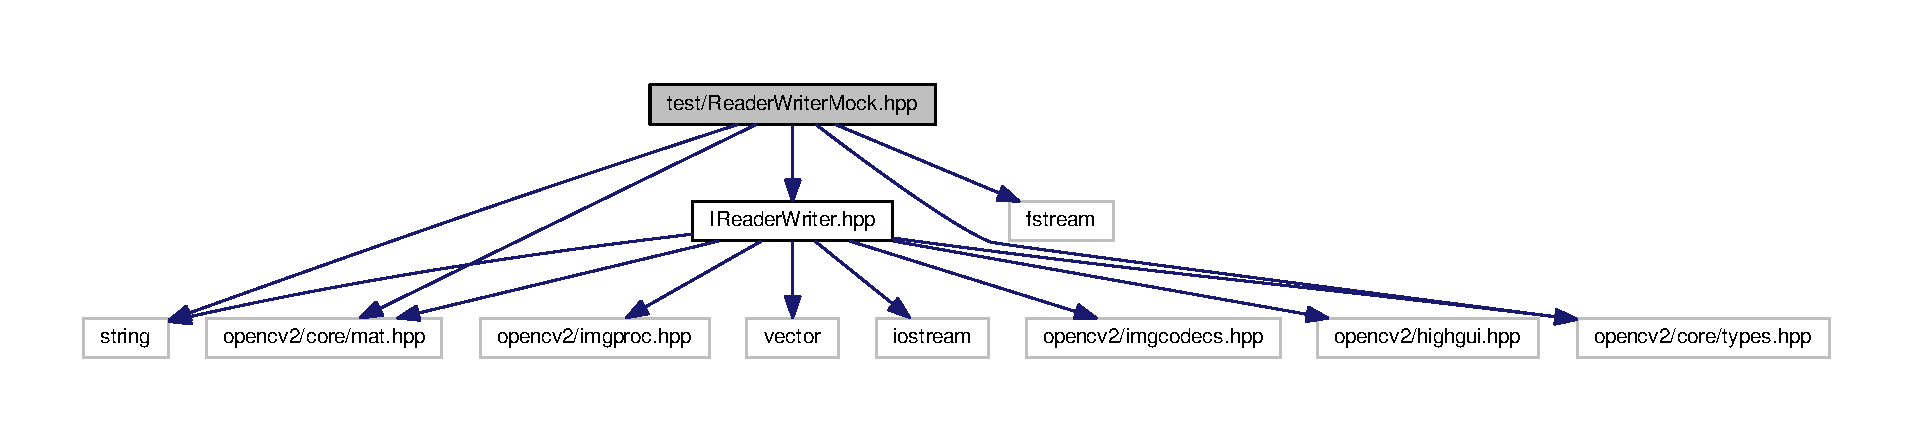
\includegraphics[width=350pt]{ReaderWriterMock_8hpp__incl}
\end{center}
\end{figure}
This graph shows which files directly or indirectly include this file\+:
\nopagebreak
\begin{figure}[H]
\begin{center}
\leavevmode
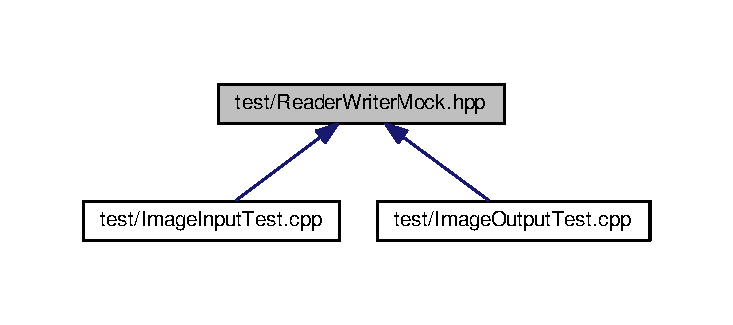
\includegraphics[width=350pt]{ReaderWriterMock_8hpp__dep__incl}
\end{center}
\end{figure}
\subsection*{Classes}
\begin{DoxyCompactItemize}
\item 
class \hyperlink{classReaderWriterMock}{Reader\+Writer\+Mock}
\end{DoxyCompactItemize}

\hypertarget{test_8cpp}{}\section{test/test.cpp File Reference}
\label{test_8cpp}\index{test/test.\+cpp@{test/test.\+cpp}}
{\ttfamily \#include $<$gtest/gtest.\+h$>$}\\*
Include dependency graph for test.\+cpp\+:
\nopagebreak
\begin{figure}[H]
\begin{center}
\leavevmode
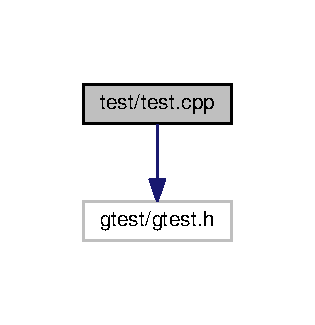
\includegraphics[width=151pt]{test_8cpp__incl}
\end{center}
\end{figure}
\subsection*{Functions}
\begin{DoxyCompactItemize}
\item 
int \hyperlink{test_8cpp_a3c04138a5bfe5d72780bb7e82a18e627}{main} (int argc, char $\ast$$\ast$argv)
\end{DoxyCompactItemize}


\subsection{Function Documentation}
\index{test.\+cpp@{test.\+cpp}!main@{main}}
\index{main@{main}!test.\+cpp@{test.\+cpp}}
\subsubsection[{\texorpdfstring{main(int argc, char $\ast$$\ast$argv)}{main(int argc, char **argv)}}]{\setlength{\rightskip}{0pt plus 5cm}int main (
\begin{DoxyParamCaption}
\item[{int}]{argc, }
\item[{char $\ast$$\ast$}]{argv}
\end{DoxyParamCaption}
)}\hypertarget{test_8cpp_a3c04138a5bfe5d72780bb7e82a18e627}{}\label{test_8cpp_a3c04138a5bfe5d72780bb7e82a18e627}

%--- End generated contents ---

% Index
\backmatter
\newpage
\phantomsection
\clearemptydoublepage
\addcontentsline{toc}{chapter}{Index}
\printindex

\end{document}
